\documentclass[12pt,t]{beamer}\usepackage[]{graphicx}\usepackage[]{color}
%% maxwidth is the original width if it is less than linewidth
%% otherwise use linewidth (to make sure the graphics do not exceed the margin)
\makeatletter
\def\maxwidth{ %
  \ifdim\Gin@nat@width>\linewidth
    \linewidth
  \else
    \Gin@nat@width
  \fi
}
\makeatother

\definecolor{fgcolor}{rgb}{0.345, 0.345, 0.345}
\newcommand{\hlnum}[1]{\textcolor[rgb]{0.686,0.059,0.569}{#1}}%
\newcommand{\hlstr}[1]{\textcolor[rgb]{0.192,0.494,0.8}{#1}}%
\newcommand{\hlcom}[1]{\textcolor[rgb]{0.678,0.584,0.686}{\textit{#1}}}%
\newcommand{\hlopt}[1]{\textcolor[rgb]{0,0,0}{#1}}%
\newcommand{\hlstd}[1]{\textcolor[rgb]{0.345,0.345,0.345}{#1}}%
\newcommand{\hlkwa}[1]{\textcolor[rgb]{0.161,0.373,0.58}{\textbf{#1}}}%
\newcommand{\hlkwb}[1]{\textcolor[rgb]{0.69,0.353,0.396}{#1}}%
\newcommand{\hlkwc}[1]{\textcolor[rgb]{0.333,0.667,0.333}{#1}}%
\newcommand{\hlkwd}[1]{\textcolor[rgb]{0.737,0.353,0.396}{\textbf{#1}}}%
\let\hlipl\hlkwb

\usepackage{framed}
\makeatletter
\newenvironment{kframe}{%
 \def\at@end@of@kframe{}%
 \ifinner\ifhmode%
  \def\at@end@of@kframe{\end{minipage}}%
  \begin{minipage}{\columnwidth}%
 \fi\fi%
 \def\FrameCommand##1{\hskip\@totalleftmargin \hskip-\fboxsep
 \colorbox{shadecolor}{##1}\hskip-\fboxsep
     % There is no \\@totalrightmargin, so:
     \hskip-\linewidth \hskip-\@totalleftmargin \hskip\columnwidth}%
 \MakeFramed {\advance\hsize-\width
   \@totalleftmargin\z@ \linewidth\hsize
   \@setminipage}}%
 {\par\unskip\endMakeFramed%
 \at@end@of@kframe}
\makeatother

\definecolor{shadecolor}{rgb}{.97, .97, .97}
\definecolor{messagecolor}{rgb}{0, 0, 0}
\definecolor{warningcolor}{rgb}{1, 0, 1}
\definecolor{errorcolor}{rgb}{1, 0, 0}
\newenvironment{knitrout}{}{} % an empty environment to be redefined in TeX

\usepackage{alltt}
% \documentclass[t]{beamer}

\usepackage{pgfpages}
\usepackage{pgffor}
%\pgfpagesuselayout{4 on 1}[a4paper,landscape]

%\pagestyle{empty} % descomentar para impresión muy blanca

\usepackage[utf8]{inputenc}
\usepackage[spanish]{babel}
\decimalpoint
\usepackage{verbatim}
\usepackage{hyperref}
\usepackage{amsfonts,amssymb,amsmath,amsthm, wasysym}
\usepackage{listings}
\usepackage[T1]{fontenc}        
\usepackage{pgf}
%\usepackage{epsdice}
\usepackage{pgfpages}
\usepackage{tikz}
%\usetikzlibrary{arrows,shapes,plotmarks,backgrounds,trees,positioning}
%\usetikzlibrary{decorations.pathmorphing,calc,snakes}
%\usepackage{marvosym}
%
\usetheme[hideothersubsections,left]{Marburg}
\usecolortheme{sidebartab}
\useinnertheme[shadow]{rounded}
% \useoutertheme[footline=empty,subsection=true,compress]{infolines}
% \useoutertheme[footline=empty,subsection=true,compress]{miniframes}
% \usefonttheme{serif}

\setbeamertemplate{caption}[numbered]
\setbeamertemplate{navigation symbols}{}


\newcommand{\red}[1]{\textcolor{red}{#1}}
\newcommand{\green}[1]{\textcolor{green}{#1}}
\newcommand{\blue}[1]{\textcolor{blue}{#1}}
\newcommand{\gray}[1]{\textcolor{gray}{#1}}
\renewcommand{\emph}[1]{{\color{red}#1}}
\newcommand{\MYhref}[3][blue]{\href{#2}{\color{#1}{#3}}}%

\setbeamertemplate{frametitle}
{\begin{centering}
\medskip
\color{blue}
\textbf{\insertframetitle}
\medskip
\end{centering}
}
\usecolortheme{rose}
\usecolortheme{dolphin}
\mode<presentation>


\newcommand{\CC}{\mathbb{C}}
\newcommand{\RR}{\mathbb{R}}
\newcommand{\ZZ}{\mathbb{Z}}
\newcommand{\NN}{\mathbb{N}}
\newcommand{\KK}{\mathbb{K}}
\newcommand{\MM}{\mathcal{M}}
%\newcommand{\dbinom}{\displaystyle\binom}

\newcommand{\limn}{{\displaystyle \lim_{n\to\infty}}}
\renewcommand{\leq}{\leqslant}
\renewcommand{\geq}{\geqslant}
\def\tendeix{{\displaystyle\mathop{\longrightarrow}_{\scriptscriptstyle
n\to\infty}}}

\newcommand{\matriu}[1]{\left(\begin{matrix} #1 \end{matrix}\right)}

% \newcommand{\qed}{\hbox{}\nobreak\hfill\vrule width 1.4mm height 1.4mm depth 0mm
%     \par \goodbreak \smallskip}
%
% %
\theoremstyle{plain}
\newtheorem{teorema}{Teorema}
\newtheorem{prop}{Propiedad}
\newtheorem{cor}{Corolario}
\theoremstyle{definition}
\newtheorem{Ejemplo}{Ejemplo}
\newtheorem{exerc}{Ejercicio}
\newtheorem{defin}{Definición}
\newtheorem{obs}{Observación}

\newcounter{seccions}
\newcommand{\seccio}[1]{\addtocounter{seccions}{1}
\medskip\par\noindent\textbf{\theseccions.
#1}\smallskip\par }

\newcommand{\EM}{\Omega}
\newcommand{\PP}{\mathcal{P}}

\title[\red{Matemáticas III GINF}]{}
\author[]{}
\date{}
\IfFileExists{upquote.sty}{\usepackage{upquote}}{}
\begin{document}
\beamertemplatedotitem

\lstset{backgroundcolor=\color{green!50}}
\lstset{breaklines=true}
\lstset{basicstyle=\ttfamily}


\section{Estimación por intervalos}

\begin{frame}
\vfill
\begin{center}
\gray{\LARGE Estimación por intervalos}
\end{center}
\vfill
\end{frame}


\subsection{Definiciones básicas}

\begin{frame}
\frametitle{El problema}
\vspace*{-1cm}

\begin{center}
\hspace*{-0.6cm}

\includegraphics[width=1.1\linewidth]{sanidade}
\end{center}
\vspace*{-1ex}

Con un estimador, estimamos el parámetro con una cierta precisión, que depende:
\medskip

\begin{itemize}
\item De la variabilidad del estimador
\medskip

\item Del tamaño de la muestra
\medskip

\item Del \emph{nivel de confianza} de la  estimación: cuan seguros  queremos estar de que la estimación es correcta
\end{itemize}
\end{frame}



\begin{frame}
\frametitle{El problema}
\vspace*{-1cm}

\begin{center}
\hspace*{-0.5cm}

\includegraphics[width=1.1\linewidth]{plagiUIB1.jpg}\medskip

\hspace*{-0.4cm}

\includegraphics[width=1.05\linewidth]{plagiUIB3.jpg}\medskip

\hspace*{-0.5cm}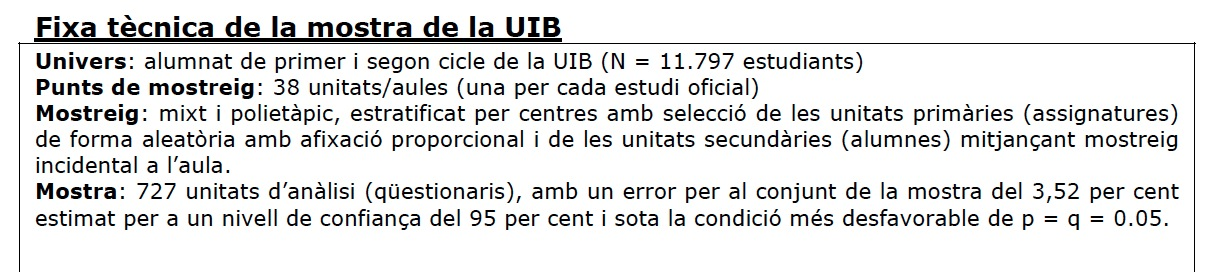
\includegraphics[width=1.1\linewidth]{plagiUIB2.jpg}
\end{center}
\vspace*{-1ex}

Por lo tanto ( y por el momento):
\begin{quote}
\red{Con 95\% de confianza podemos afirmar que entre un 73.1\% y un 80.1\% de los estudiantes de la UIB aceptan \ldots}
\end{quote}
\end{frame}


\begin{frame}
\frametitle{El problema}
\vspace*{-0.5cm}

\begin{center}

\includegraphics[width=1\linewidth]{EPA3}
\end{center}
\end{frame}

\begin{frame}
\frametitle{Definiciones básicas}

En la \blue{Encuesta de Población Activa} (\blue{EPA}):

\begin{center}
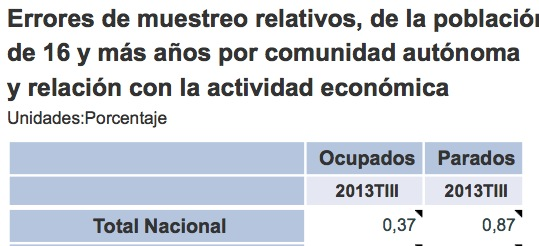
\includegraphics[width=0.6\linewidth]{EPA1}

{\scriptsize \url{http://www.ine.es/jaxi/tabla.do?per=03&type=db&divi=EPA&idtab=313}}
\medskip

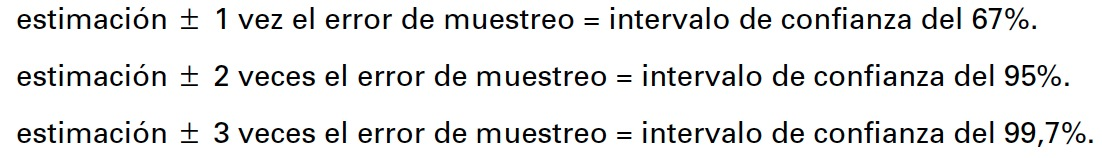
\includegraphics[width=\linewidth]{EPA2}


{\scriptsize \url{http://www.ine.es/docutrab/eval_epa/evaluacion_epa04.pdf}}
\end{center}
\end{frame}

\begin{frame}
\frametitle{El problema}
\vspace*{-2ex}

\blue{EPA de octubre de 2013}: \smallskip
\begin{itemize}
\item El número  estimado de parados a nivel nacional fue del  5\,904\,700 \smallskip

\item El error de muestreo fue de un 0.87\% \smallskip

\item Por lo tanto, estamos bastante seguros (nivel de confianza del 95\%) de que el número de parados estaba entre
$$
\begin{array}{rl}
\hspace*{-2ex} 5\,904\,700\!-\! 2\!\cdot \! 0.0087\!\cdot\! 5\,904\,700 & \hspace*{-1ex}=\! 5\,904\,700\!-\! 102\,742\\ &  \hspace*{-1ex}=\! 5\,801\,958\quad \mbox{ y}\\
\hspace*{-2ex} 5\,904\,700\!+\!2\!\cdot\! 0.0087\!\cdot\! 5\,904\,700 & \hspace*{-1ex}=\! 5\,904\,700\!+\! 102\,742\\ & \hspace*{-1ex}=\! 6\,007\,442
 \end{array}
 $$
 
 \item La EPA de junio del 2013 había estimado el número de parados  en  5\,977\,500
 \smallskip
 
 \item \red{No hay evidencia de que  el paro bajase}
 \end{itemize}
\end{frame}


\begin{frame}
\frametitle{Definiciones básicas}

Una \emph{estimación por intervalos} de un parámetro poblacional es una regla para calcular, a partir de una muestra,
un intervalo en el que, con una cierta probabilidad (\emph{nivel de confianza}), se encuentra el  valor verdadero del parámetro
\bigskip

Estas reglas definirán,  a su vez, \emph{estimadores}

\end{frame}



\begin{frame}
\frametitle{Ejemplos}


\blue{Ejemplo:} 
Hemos escogido al azar 50 estudiantes de grado de la UIB, hemos calculada sus notas medias de las asignaturas del primer semestre, y la media de estas medias ha sido un 6.3, con una varianza muestral de 1.8.\medskip

Determinar un intervalo del que podamos afirmar con probabilidad 95\% que contiene la media real de las notas medias de los estudiantes de grado de la UIB este primer semestre.
\end{frame}


\begin{frame}
\frametitle{Ejemplos}

\blue{Ejemplo:} En un experimento en el que se ha medido la tasa oficial  de  alcoholemia en sangre a 40 varones (sobrios) después de tomar 3 cañas de cerveza de 330 ml.
La media y la desviación típica de esta tasa han sido
$$
\overline{x}=0.7,\quad \widetilde{s}=0.1
$$
Determinar un intervalo que podamos afirmar con probabilidad 95\% que contiene la tasa de alcoholemia media en sangre de una varón  después de beber 3  cañas de cerveza de 330ml.
\end{frame}




\begin{frame}
\frametitle{Definiciones básicas}

Dado un parámetro $\theta$, el intervalo $]A,B[$ es un \emph{intervalo de confianza} del
$(1-\alpha)\cdot 100\% $ para al parámetro $\theta$ cuando
$$
P(A<\theta<B)=1-\alpha
$$
El valor $(1-\alpha)\cdot 100\% $ (o contiene solo el $1-\alpha$) recibe el nombre de \emph{nivel de confianza} 
\medskip

El valor $\alpha$ recibe el nombre de \emph{nivel de significación}
\medskip 


\blue{Ejemplo:} $]A,B[$ es un intervalo de confianza del $95\%$ (o de nivel de significación de 0.05) si
$$
P(A<\theta<B)=0.95
$$
\end{frame}




\begin{frame}
\frametitle{Definiciones básicas}

\emph{Por defecto}, buscaremos  intervalos bilaterales tales que la \emph{cola} de probabilidad sobrante $\alpha$ se reparta por igual a cada lado  del intervalo:
$$
P(\theta<A)=P(\theta>B)=\frac{\alpha}{2}
$$
\begin{center}
\begin{tikzpicture}[thick,scale=0.8]%[>=stealth]%,yscale=0.5,xscale=0.7]
\draw (0,0)--(10,0);
\draw (3,0.3)--(3,-0.3);
\draw (7,0.3)--(7,-0.3);
\draw(3,-0.6) node {\small $A$}; 
\draw (7,-0.6) node {\small $B$}; 
\draw[red] (8.5,-0.3) node {\small $\alpha/2$}; 
\draw[red] (1.5,-0.3) node {\small $\alpha/2$}; 
\draw[red] (5,-0.3) node {\small $1-\alpha$}; 
\end{tikzpicture}
\end{center}


\blue{Ejemplo:} Para buscar  un intervalo de confianza  $]A,B[$ del $95\%$, buscaremos $A,B$ de manera que 
$$
P(\theta<A)=0.025\quad\mbox{ y }\quad P(\theta>B)=0.025
$$


\end{frame}

\subsection{$\mu$ de población normal con $\sigma$ conocida}
\begin{frame}
\frametitle{Ejemplo: $\mu$ de población normal con $\sigma$ conocida}

Sea $X$ una v.a. normal con media poblacional $\mu$ desconocida y desviación típica poblacional $\sigma$ conocida (a la práctica, usualmente, \emph{estimada en un experimento anterior})
\medskip

Sea $X_1,\ldots,X_n$ una m.a.s. de $X$, con media muestral $\overline{X}$
\medskip

Queremos determinar un intervalo de confianza para a $\mu$ con un cierto nivel de confianza (digamos, 97.5\%):  un intervalo $]A,B[$ tal que
$$
P(A<\mu<B)=0.975
$$


\end{frame}

\begin{frame}
\frametitle{Ejemplo: $\mu$ de población normal con $\sigma$ conocida}

Bajo estas  condiciones, sabemos que 
$$
Z=\frac{\overline{X}-\mu}{\sigma/\sqrt{n}}
$$
sigue una distribución normal estándar
\medskip

Comencemos calculando un intervalo centrado en $0$ en el que   $Z$ 
tenga probabilidad $0.975$:
$$
\begin{array}{l}
0.975\!=\! P(-\delta<Z<\delta)\!=\!F_{Z}(\delta)\!-\!F_{Z}(-\delta)\!=\!
2 F_{Z}(\delta)\!-\!1\\[2ex]
F_{Z}(\delta)=\dfrac{1.975}{2}=0.9875\Rightarrow
\delta=\texttt{qnorm(0.9875)}=2.24
\end{array}
$$
\end{frame}


\begin{frame}
\frametitle{Ejemplo: $\mu$ de población normal con $\sigma$ conocida}
Por lo tanto
$$
P(-2.24<Z<2.24)=0.975
$$
Substituyendo $Z=\dfrac{\overline{X}-\mu}{\sigma/\sqrt{n}}$
$$
\begin{array}{c}
P\left(-2.24<\dfrac{\overline{X}-\mu}{\sigma/\sqrt{n}}
<2.24\right)=0.975\\[3ex]
P\left(\overline{X} -2.24 \dfrac{\sigma}{\sqrt{n}}< \mu< \overline{X}+
2.24\dfrac{\sigma}{\sqrt{n}}\right)=0.975
\end{array}
$$
\end{frame}

\begin{frame}
\frametitle{Ejemplo: $\mu$ de población normal con $\sigma$ conocida}
Por  lo tanto, la probabilidad que la media  $\mu$ de $X$ 
se encuentre dentro del intervalo
$$
\left]\overline{X} -2.24 \frac{\sigma}{\sqrt{n}},
\overline{X}+ 2.24\frac{\sigma}{\sqrt{n}}
\right[
$$
es $0.975$: es un intervalo de confianza  del 97.5\%
%\pause
\medskip

\red{Además tenemos que:}
\begin{itemize}
\item Está centrado en $\overline{X}$
\medskip

\item El 0.025 de probabilidad restante  está repartido por igual en los dos extremos del intervalo
\end{itemize}
\end{frame}

\begin{frame}
\frametitle{Ejemplo: $\mu$ de población normal con $\sigma$ conocida}


\begin{itemize}
\item \blue{Como  estimador:} Un 97.5\% de las veces  que tomemos una muestra de tamaño $n$ de $X$, el verdadero valor de $\mu$ caerá dentro de este intervalo 
\medskip

\item \blue{Para una muestra concreta:} La probabilidad de que la media  $\mu$ de la población que ha producido esta muestra, esté en este intervalo concreto, es del 97.5\%
\medskip

\item \blue{En ocasiones lo entenderemos como}:  ``La probabilidad de que $\mu$ esté en este intervalo es del 97.5\%''
\medskip

\item \blue{Pero la frase anterior es mentira} (\emph{es un abuso de lenguaje}): La $\mu$ concreta es un valor fijo, por lo  tanto  que pertenezca o   no a este intervalo concreto tiene probabilidad 1 (si   pertenece) y 0 (si no  pertenece) 
\end{itemize}


\end{frame}



\begin{frame}
\frametitle{I.C. para $\mu$ de población normal con $\sigma$ conocida}
\vspace*{-3ex}

\begin{teorema}
Sea $X\sim N(\mu,\sigma)$ con $\mu$ desconocida y $\sigma$ conocida.
\medskip

Tomamos una m.a.s. de $X$ de medida $n$, con media $\overline{X}$.
\medskip

Un intervalo de confianza  del $(1-\alpha)\cdot 100\%$ para $\mu$  es
$$
\left]\overline{X} -z_{1-\frac{\alpha}{2}} \frac{\sigma}{\sqrt{n}}, \overline{X}+z_{1-\frac{\alpha}{2}}\frac{\sigma}{\sqrt{n}}
\right[
$$
donde $z_{1-\frac{\alpha}{2}}$ es el $(1-\frac{\alpha}{2})$-cuantil de la normal  estándar $Z$ (es decir, $z_{1-\frac{\alpha}{2}}=F_Z^{-1}(1-\frac{\alpha}{2})$, o $P(Z\leq z_{1-\frac{\alpha}{2}})=1-\frac{\alpha}{2}$)
\end{teorema}

%(Recordau que $F_Z^{-1}(\frac{\alpha}{2})=-F_Z^{-1}(1-\frac{\alpha}{2})$)

\end{frame}


\begin{frame}
\frametitle{I.C. para $\mu$ de población normal con $\sigma$ conocida}

Si $X$ es normal con $\sigma$ conocida, un intervalo de confianza  I.C. para $\mu$ de población normal con $\sigma$ conocida $\mu$ del $(1-\alpha)\cdot 100\%$ es
$$
\red{\overline{X} \pm z_{1-\frac{\alpha}{2}} \frac{\sigma}{\sqrt{n}}}:=\left]\overline{X} -z_{1-\frac{\alpha}{2}} \frac{\sigma}{\sqrt{n}}, \overline{X}+z_{1-\frac{\alpha}{2}}\frac{\sigma}{\sqrt{n}}
\right[
$$
Observad que está centrado   en $\overline{X}$
\begin{center}
\begin{tabular}{c|c|c}
\blue{confianza  $1-\alpha$} & \blue{Significación $\alpha$} & \blue{$z_{1-\frac{\alpha}{2}}$}\\
 \hline
0.900\ & 0.100 &1.64 \\   
0.950 & 0.050 & 1.96\\
0.975 & 0.025 & 2.24 \\
0.990 & 0.010 & 2.58
\end{tabular}
\end{center}

\end{frame}

\begin{frame}[fragile]
\frametitle{I.C. para $\mu$ de población normal con $\sigma$ conocida}
\vspace*{-4ex}

\begin{knitrout}\footnotesize
\definecolor{shadecolor}{rgb}{0.969, 0.969, 0.969}\color{fgcolor}\begin{kframe}
\begin{alltt}
\hlstd{ICZ}\hlkwb{=}\hlkwa{function}\hlstd{(}\hlkwc{x}\hlstd{,}\hlkwc{sigma}\hlstd{,}\hlkwc{alpha}\hlstd{)\{}
  \hlkwd{c}\hlstd{(}\hlkwd{mean}\hlstd{(x)}\hlopt{-}\hlkwd{qnorm}\hlstd{(}\hlnum{1}\hlopt{-}\hlstd{alpha}\hlopt{/}\hlnum{2}\hlstd{)}\hlopt{*}\hlstd{sigma}\hlopt{/}\hlkwd{sqrt}\hlstd{(}\hlkwd{length}\hlstd{(x)),}
  \hlkwd{mean}\hlstd{(x)}\hlopt{+}\hlkwd{qnorm}\hlstd{(}\hlnum{1}\hlopt{-}\hlstd{alpha}\hlopt{/}\hlnum{2}\hlstd{)}\hlopt{*}\hlstd{sigma}\hlopt{/}\hlkwd{sqrt}\hlstd{(}\hlkwd{length}\hlstd{(x)))\}}
\hlkwd{set.seed}\hlstd{(}\hlnum{5}\hlstd{)}
\hlstd{mu}\hlkwb{=}\hlnum{1.5}\hlstd{; sigma}\hlkwb{=}\hlnum{1}\hlstd{; alpha}\hlkwb{=}\hlnum{0.05}
\hlstd{Población}\hlkwb{=}\hlkwd{rnorm}\hlstd{(}\hlnum{10}\hlopt{^}\hlnum{6}\hlstd{,mu,sigma)}
\hlstd{M}\hlkwb{=}\hlkwd{replicate}\hlstd{(}\hlnum{100}\hlstd{,}\hlkwd{ICZ}\hlstd{(}\hlkwd{sample}\hlstd{(Población,}\hlnum{50}\hlstd{,}\hlkwc{replace}\hlstd{=T),}
 \hlstd{sigma,alpha))}
\hlkwd{plot}\hlstd{(}\hlnum{1}\hlopt{:}\hlnum{10}\hlstd{,}\hlkwc{type}\hlstd{=}\hlstr{"n"}\hlstd{,}\hlkwc{xlim}\hlstd{=}\hlkwd{c}\hlstd{(}\hlnum{1.2}\hlstd{,}\hlnum{1.8}\hlstd{),}\hlkwc{ylim}\hlstd{=}\hlkwd{c}\hlstd{(}\hlnum{0}\hlstd{,}\hlnum{100}\hlstd{),}
\hlkwc{xlab}\hlstd{=}\hlstr{"Valores"}\hlstd{,}\hlkwc{ylab}\hlstd{=}\hlstr{"Replicaciones"}\hlstd{)}
\hlstd{seg.int}\hlkwb{=}\hlkwa{function}\hlstd{(}\hlkwc{i}\hlstd{)\{color}\hlkwb{=}\hlstr{"grey"}\hlstd{;}
  \hlkwa{if}\hlstd{((mu}\hlopt{<}\hlstd{M[}\hlnum{1}\hlstd{,i])} \hlopt{|} \hlstd{(mu}\hlopt{>}\hlstd{M[}\hlnum{2}\hlstd{,i]))\{color} \hlkwb{=} \hlstr{"red"}\hlstd{\}}
  \hlkwd{segments}\hlstd{(M[}\hlnum{1}\hlstd{,i],i,M[}\hlnum{2}\hlstd{,i],i,}\hlkwc{col}\hlstd{=color,}\hlkwc{lwd}\hlstd{=}\hlnum{3}\hlstd{)\}}
\hlkwd{invisible}\hlstd{(}\hlkwd{sapply}\hlstd{(}\hlnum{1}\hlopt{:}\hlnum{100}\hlstd{,}\hlkwc{FUN}\hlstd{=seg.int))}
\hlkwd{abline}\hlstd{(}\hlkwc{v}\hlstd{=mu,}\hlkwc{lwd}\hlstd{=}\hlnum{3}\hlstd{)}
\end{alltt}
\end{kframe}
\end{knitrout}

\end{frame}

\begin{frame}

\frametitle{I.C. para $\mu$ de población normal con $\sigma$ conocida}
\vspace*{-1cm}

% \begin{center}
% 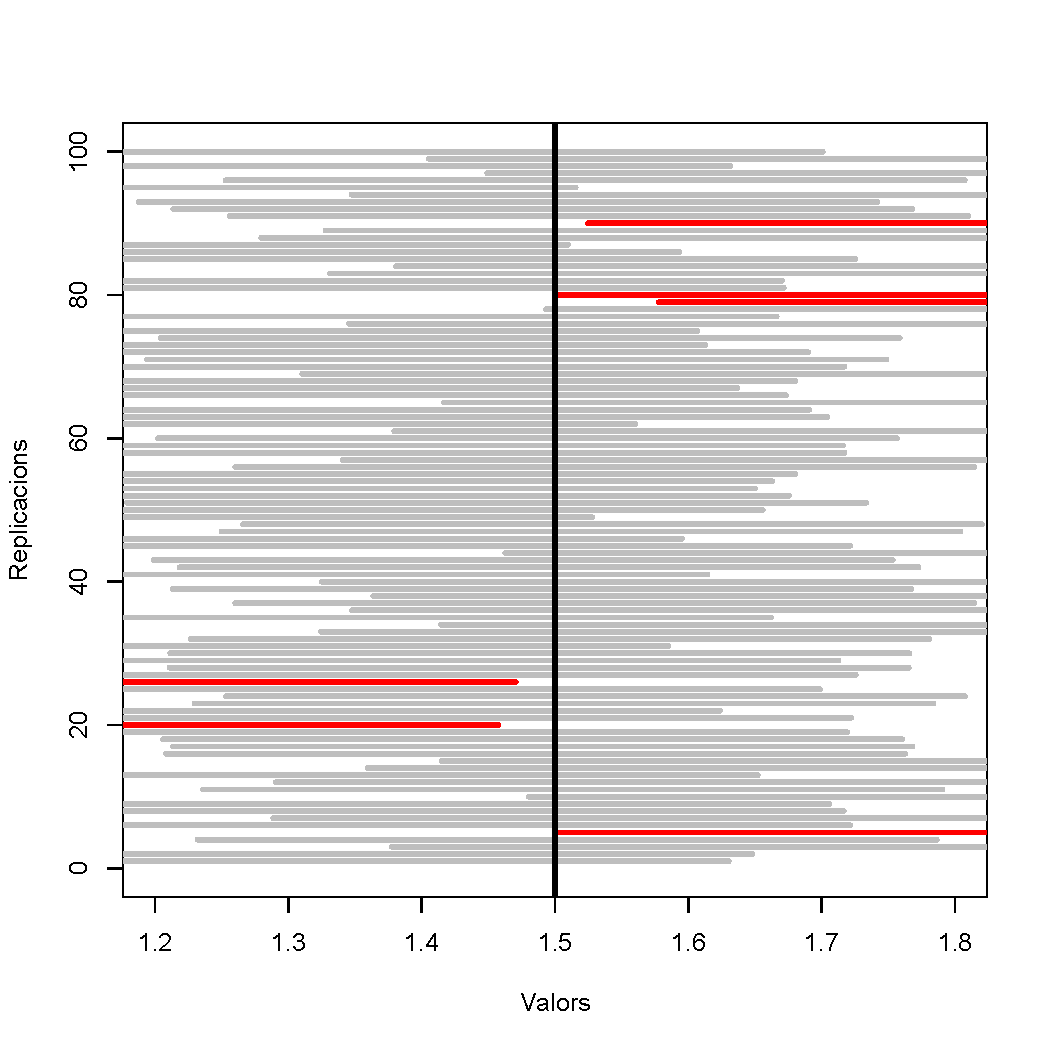
\includegraphics[width=0.9\linewidth]{intervals1}
% \end{center}
\begin{knitrout}
\definecolor{shadecolor}{rgb}{0.969, 0.969, 0.969}\color{fgcolor}
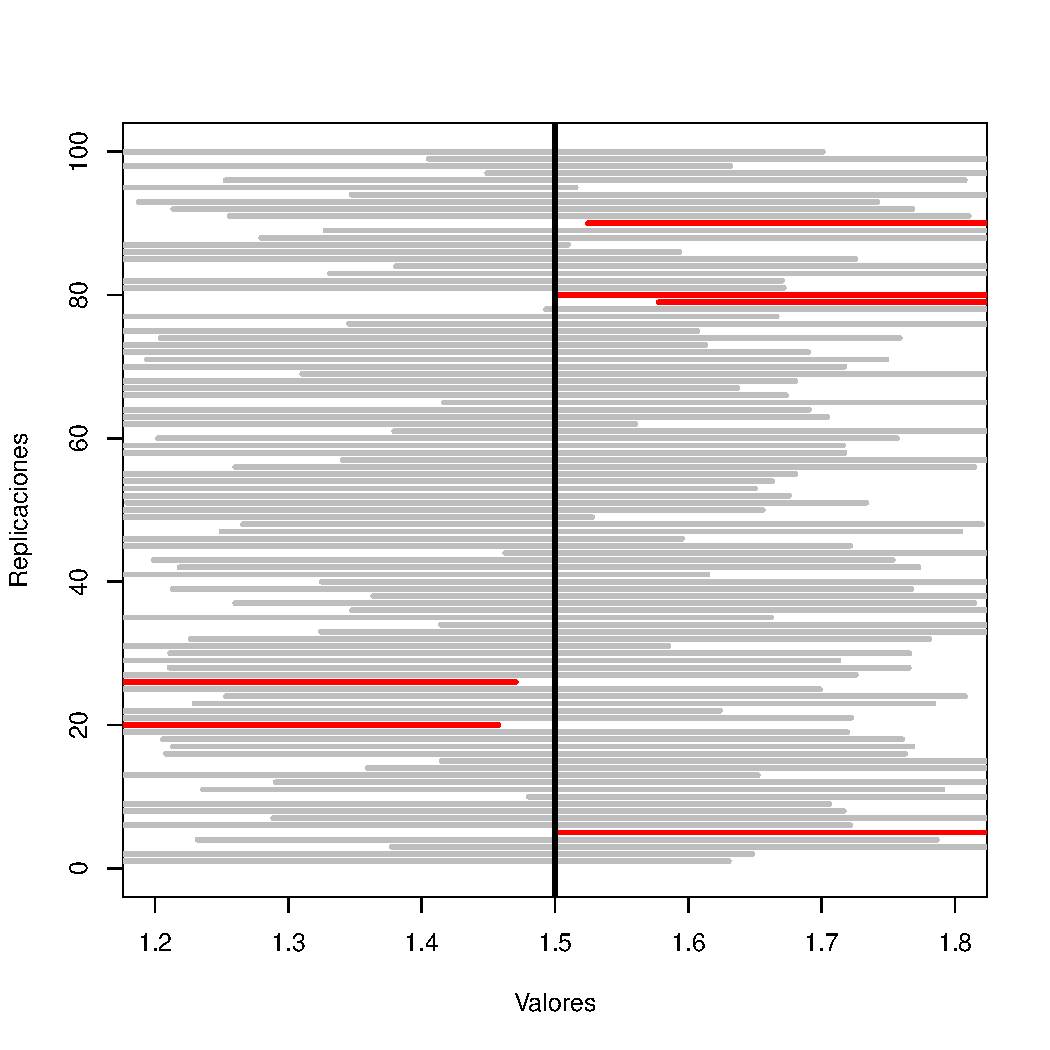
\includegraphics[width=0.9\linewidth]{figure/plot_intervalos-1} 

\end{knitrout}




\end{frame}

\begin{frame}[fragile]
\frametitle{I.C. para $\mu$ de población normal con $\sigma$ conocida}

\begin{block}{\red{¡Atención!}}
De media, un $\alpha\cdot 100\%$ de las veces, un intervalo de confianza  del $(1-\alpha)\cdot 100\%$  no contendrá el valor real del parámetro 
\end{block}

\blue{Ejemplo}: De media, un 5\% de las veces un intervalo de confianza  del 95\% no contendrá el valor real del parámetro

\end{frame}




\begin{frame}
\frametitle{Ejemplo}
\red{$\displaystyle
\left]\overline{X} -z_{1-\frac{\alpha}{2}} \frac{\sigma}{\sqrt{n}}, \overline{X}+z_{1-\frac{\alpha}{2}}\frac{\sigma}{\sqrt{n}}
\right[$}
\medskip


Tomamos una m.a.s. de  tamaño  $n=16$ de una v.a. normal con $\sigma=4$ y $\mu$ desconocida. La media   de la m.a.s. es
$\overline{x}=20$.
\medskip

\blue{Calculad un intervalo de confianza  del 97.5\%  para $\mu$ de  una población normal con $\sigma$ conocida}
%\pause
$$
\left] 20-2.24\cdot \frac{4}{\sqrt{16}} ,
20+2.24\cdot \frac{4}{\sqrt{16}}
\right[
=]17.76,22.24[
$$

La probabilidad que un parámetro $\mu$ que haya producido la muestra esté en este intervalo  es $0.975$
%\pause
\medskip

\textsl{``La probabilidad que el parámetro $\mu$  de la población que ha producido la muestra este  en este intervalo  es $0.975$''}


\end{frame}


\begin{frame}[fragile]
\frametitle{Ejemplo}
Queremos que analizar un sensor que mide la temperatura de un procesador en grados centígrados \footnote{En concreto un \emph{Intel Core i7-2600K}} que tiene 	como temperatura normal de  $32^{\circ}$ a $40^{\circ}$. Para saber si está bien calibrado, diseñamos un experimento en el que ponemos  el procesador el procesador en las mismas condiciones y  tomamos 40 muestras de su temperatura.
Los resultados son los siguientes:

\begin{knitrout}\small
\definecolor{shadecolor}{rgb}{0.969, 0.969, 0.969}\color{fgcolor}\begin{kframe}
\begin{alltt}
\hlstd{temperatura}\hlkwb{=}\hlkwd{c}\hlstd{(}\hlnum{36}\hlstd{,}\hlnum{35}\hlstd{,}\hlnum{38}\hlstd{,}\hlnum{38}\hlstd{,}\hlnum{36}\hlstd{,}\hlnum{37}\hlstd{,}\hlnum{38}\hlstd{,}\hlnum{36}\hlstd{,}\hlnum{37}\hlstd{,}\hlnum{36}\hlstd{,}
              \hlnum{37}\hlstd{,}\hlnum{37}\hlstd{,}\hlnum{34}\hlstd{,}\hlnum{38}\hlstd{,}\hlnum{35}\hlstd{,}\hlnum{37}\hlstd{,}\hlnum{36}\hlstd{,}\hlnum{36}\hlstd{,}\hlnum{34}\hlstd{,}\hlnum{38}\hlstd{,}
              \hlnum{36}\hlstd{,}\hlnum{37}\hlstd{,}\hlnum{35}\hlstd{,}\hlnum{35}\hlstd{,}\hlnum{35}\hlstd{,}\hlnum{35}\hlstd{,}\hlnum{36}\hlstd{,}\hlnum{36}\hlstd{,}\hlnum{36}\hlstd{,}\hlnum{35}\hlstd{,}
              \hlnum{36}\hlstd{,}\hlnum{35}\hlstd{,}\hlnum{34}\hlstd{,}\hlnum{34}\hlstd{,}\hlnum{37}\hlstd{,}\hlnum{37}\hlstd{,}\hlnum{35}\hlstd{,}\hlnum{36}\hlstd{,}\hlnum{34}\hlstd{,}\hlnum{36}\hlstd{)}
\hlkwd{mean}\hlstd{(temperatura)}
\end{alltt}
\begin{verbatim}
## [1] 35.975
\end{verbatim}
\end{kframe}
\end{knitrout}

\end{frame}

\begin{frame}[fragile]
\frametitle{Ejemplo}
\vspace*{-3ex}

\blue{Supongamos  que las medidas de nuestro sensor siguen  una distribución normal con varianza poblacional conocida $\sigma^2=1.44$. Calculad un intervalo de confianza  del 90\% para al resultado medio de la temperatura del procesador.}
%\pause
\medskip

Tenemos las siguientes condiciones:
\begin{itemize}
\item Población normal con $\sigma=\sqrt{1.44}=1.2$ conocida
\item Muestra aleatoria simplede  tamaño  $n=40$
\item Media de la muestra  $\overline{x}=35.975$
\item $1-\alpha=0.9\Rightarrow \alpha=0.1\Rightarrow 1-\frac{\alpha}{2}=0.95$
\item $z_{0.95}\approx 1.64$
\begin{itemize}
\item Con la tabla de $Z$, $P(Z\leq 1.64)=0.9495\approx 0.95$
\item Con R
\begin{knitrout}
\definecolor{shadecolor}{rgb}{0.969, 0.969, 0.969}\color{fgcolor}\begin{kframe}
\begin{alltt}
\hlkwd{qnorm}\hlstd{(}\hlnum{0.95}\hlstd{)}
\end{alltt}
\begin{verbatim}
## [1] 1.644854
\end{verbatim}
\end{kframe}
\end{knitrout}
\end{itemize}
\end{itemize}

\end{frame}


\begin{frame}
\frametitle{Ejemplo}
Aplicamos la fórmula
$$
\overline{X}\pm z_{1-\frac{\alpha}{2}} \frac{\sigma}{\sqrt{n}}
$$
con
$$
\overline{x}=35.975, z_{0.95}=1.64, \sigma=\sqrt{1.44}=1.2, n=40
$$

Obtenemos que el intervalo de confianza  del 90\% es 

$$
35.975\pm 1.64\cdot\frac{1.2}{\sqrt{40}}=
]34.991 , 36.959[
$$

\end{frame}


\begin{frame}
\frametitle{Amplitud}

La \emph{amplitud} $A$ de un intervalo de confianza  
$$
\left]\overline{X} -z_{1-\frac{\alpha}{2}} \frac{\sigma}{\sqrt{n}}, \overline{X}+z_{1-\frac{\alpha}{2}}\frac{\sigma}{\sqrt{n}}
\right[
$$
es
$$
\begin{array}{rl}
\red{A}& \displaystyle =\overline{X}+ z_{1-\frac{\alpha}{2}}\frac{\sigma}{\sqrt{n}}-\Big(\overline{X} -z_{1-\frac{\alpha}{2}}\frac{\sigma}{\sqrt{n}}\Big)\\[2ex] & \displaystyle =\red{2\cdot z_{1-\frac{\alpha}{2}}\frac{\sigma}{\sqrt{n}}}
\end{array}
$$
%\end{frame}

El \emph{error máximo}, al nivel de confianza  $(1-\alpha)$, que cometemos al estimar $\mu$
por  $\overline{X}$ es la mitad de la amplitud, 
$$
\red{z_{1-\frac{\alpha}{2}}\frac{\sigma}{\sqrt{n}}}
$$
\end{frame}

\begin{frame}
\frametitle{Amplitud}

La \emph{Amplitud} $A$ del intervalo de confianza 
$$
\left]\overline{X} -z_{1-\frac{\alpha}{2}} \frac{\sigma}{\sqrt{n}}, \overline{X}+z_{1-\frac{\alpha}{2}}\frac{\sigma}{\sqrt{n}}
\right[
$$
es
$$
A= 2\cdot z_{1-\frac{\alpha}{2}}\frac{\sigma}{\sqrt{n}}
$$

\blue{Observaciones}
\begin{itemize}
\item I.C. para $\mu$ de una población normal con $\sigma$ conocida $n$ y $\alpha$ fijos, si $\sigma$ crece,
 $A$ crece
\smallskip

\item I.C. para $\mu$ de población normal con $\sigma$ conocida $\sigma$ y $\alpha$ fijos, si $n$
crece,  $A$ decrece
\smallskip

\item I.C. para $\mu$ de población normal con $\sigma$ conocida $\sigma$ y $n$ fijos, si
$1-\alpha$ crece, $A$ crece
\end{itemize}
\end{frame}




\begin{frame}
\frametitle{Amplitud}

Si queremos calcular el   tamaño  $n$ de la muestra para asegurar que el intervalo de confianza  para $\mu$ al nivel de confianza $(1-\alpha)$ tenga una amplitud prefijada máxima $A_0$ (o un
error máximo $A_0/2$), podemos despejar el tamaño muestral  $n$ de:
$$
A_0\geq 2z_{1-\frac{\alpha}{2}}\frac{\sigma}{\sqrt{n}}\Rightarrow
n\geq \left( 2 z_{1-\frac{\alpha}{2}}\frac{\sigma}{A_0}
\right)^2
$$
Dada $A_0$, tomaremos
$$
\red{n=\left\lceil \left( 2 z_{1-\frac{\alpha}{2}}\frac{\sigma}{A_0}
\right)^2\right\rceil}
$$

\end{frame}


\begin{frame}
\frametitle{Ejemplo}

\blue{Recordemos  que las medidas de nuestro sensor  de temperatura seguían una distribución normal con varianza poblacional conocida $\sigma^2=1.44$,  $\sigma=1.2$}
\medskip

\blue{¿Cuántas medidas tendríamos que tomar para obtener la  temperatura media  con un error máximo de $0.05^{\circ}$ al nivel de confianza del 90\%?}
%\pause
$$
n=\left\lceil \left( 2 z_{1-\frac{\alpha}{2}}\frac{\sigma}{A_0}
\right)^2\right\rceil$$
donde 
$$
\frac{A_0}{2}=0.05,\quad z_{1-\frac{\alpha}{2}}=1.64,\quad \sigma=0.1
$$
Obtenemos $n= \lceil10.76\rceil= 11$
\end{frame}



\subsection{$\mu$ de población normal con $\sigma$ desconocida}

\begin{frame}
\frametitle{Distribución $t$ de Student}


Sea $X\sim N(\mu,\sigma)$
\medskip

Sea $X_1,\ldots,X_n$ una m.a.s. de $X$, con media   $\overline{X}$ y desviación típica muestral $\widetilde{S}_{X}$
\medskip

\begin{teorema}
En estas condiciones, la v.a.
$$
t=\frac{\overline{X}-\mu}{\widetilde{S}_{X}/\sqrt{n}}
$$
sigue una distribución \emph{$t$ de Student} con $n-1$ grados de libertad, \red{$t_{n-1}$}
\end{teorema}
\medskip

\red{$\widetilde{S}_{X}/\sqrt{n}$}: el \emph{error muestral}, estima el error estándar $\sigma/\sqrt{n}$
\end{frame}



\begin{frame}
\frametitle{distribución $t$ de Student}


La distribución $t$ de Student con $\nu$ grados de libertad, \red{$t_{\nu}$}:
\medskip

\begin{itemize}
\item  Tiene  densidad
$$
f_{t_\nu}(x) = \frac{\Gamma(\frac{\nu+1}{2})} {\sqrt{\nu\pi}\,\Gamma(\frac{\nu}{2})} \Big(1+\frac{x^2}{\nu} \Big)^{-\frac{\nu+1}{2}}
$$
donde $\Gamma(x)=\int_{0}^{\infty} t^{x-1}e^{-t}\, dt$ si $x> 0$. 
\bigskip

\item La distribución está tabulada (\emph{las tablas en el moodle de la asignatura}), y con R es \texttt{t}.
\end{itemize}
\end{frame}




\begin{frame}
\frametitle{Distribución $t$ de Student}

Sea $t_{\nu}$ una v.a. que sigue la distribución $t$ de
Student con $\nu$ grados de libertad
\medskip

\begin{itemize}
\item $E(t_{\nu})=0$  si $\nu>1$ y $Var(t_{\nu})=\dfrac{\nu}{\nu-2}$ si $\nu>2$
\medskip

\item Su  función de distribución es simétrica respecto de $E(t_{\nu})=0$ (como la de una $N(0,1)$):
$$
P(t_{\nu}\leq -x)=P(t_{\nu}\geq x)=1-P(t_{\nu}\leq x)
$$

\item Si $\nu$ es grande, su distribución es aproximadamente la de $N(0,1)$ (pero con más varianza: un poco más aplastada)
\end{itemize}

\end{frame}

\begin{frame}[fragile]
\frametitle{Distribución $t$ de Student}
%\vspace*{-1cm}

%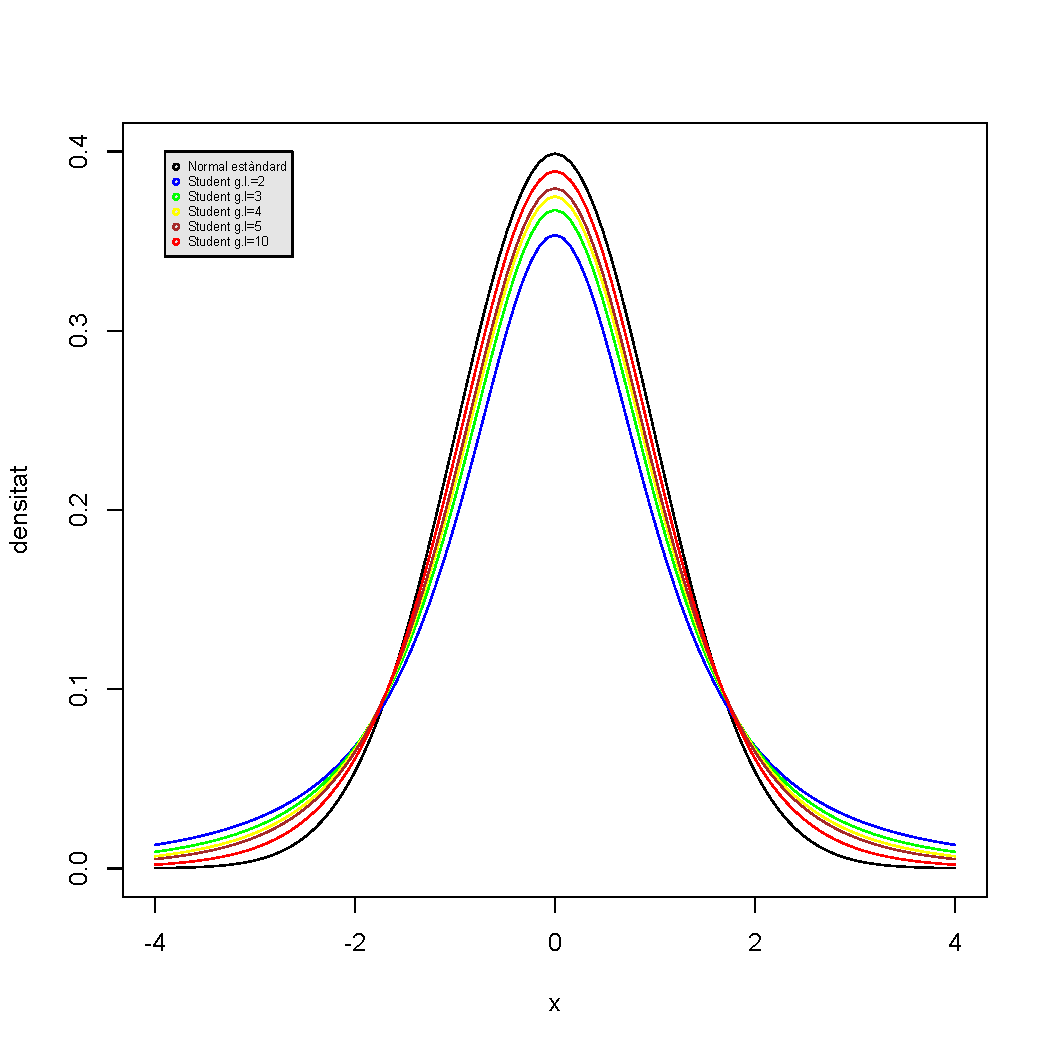
\includegraphics[width=0.95\linewidth]{tstud-div.pdf}
EL siguiente código dibuja distintas densidades de la distribución $t$ de Student
{\small
\begin{verbatim}
curve(dnorm(x, 0, 1), xlim = c(-4, 4),
      ylim = c(0, 0.4), col = "black",
      ylab = "densidad", xlab = "x")
legend("topleft",  
        legend = c("Normal estándar", "Student gl=2",
                   "Student gl=3",  "Student gl=4", 
                   "Student gl=5",  "Student gl=10"),
        fill = c("black", "brown", "green", "tomato",
                "pink", "darkblue"), cex = 0.8)
curve(dt(x, df = 2), col = "brown", add = TRUE)
curve(dt(x, df = 3), col = "green", add = TRUE)
curve(dt(x, df = 4), col = "tomato", add = TRUE)
curve(dt(x, df = 5), col = "pink", add = TRUE)
curve(dt(x, df = 10), col = "darkblue", add = TRUE)
\end{verbatim}
}
\end{frame}

\begin{frame}
\frametitle{Distribución $t$ de Student}
\vspace*{-1cm}

%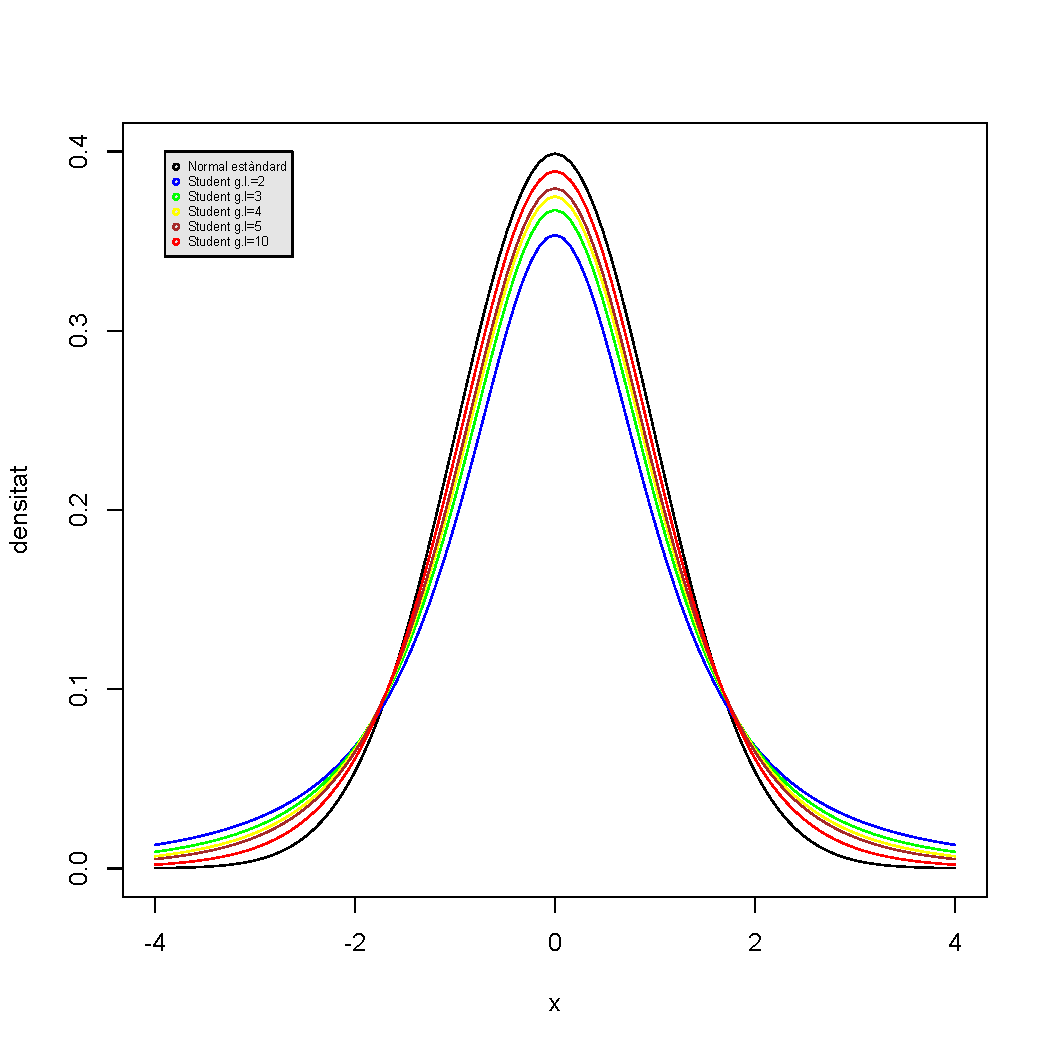
\includegraphics[width=0.95\linewidth]{tstud-div.pdf}

\begin{knitrout}
\definecolor{shadecolor}{rgb}{0.969, 0.969, 0.969}\color{fgcolor}
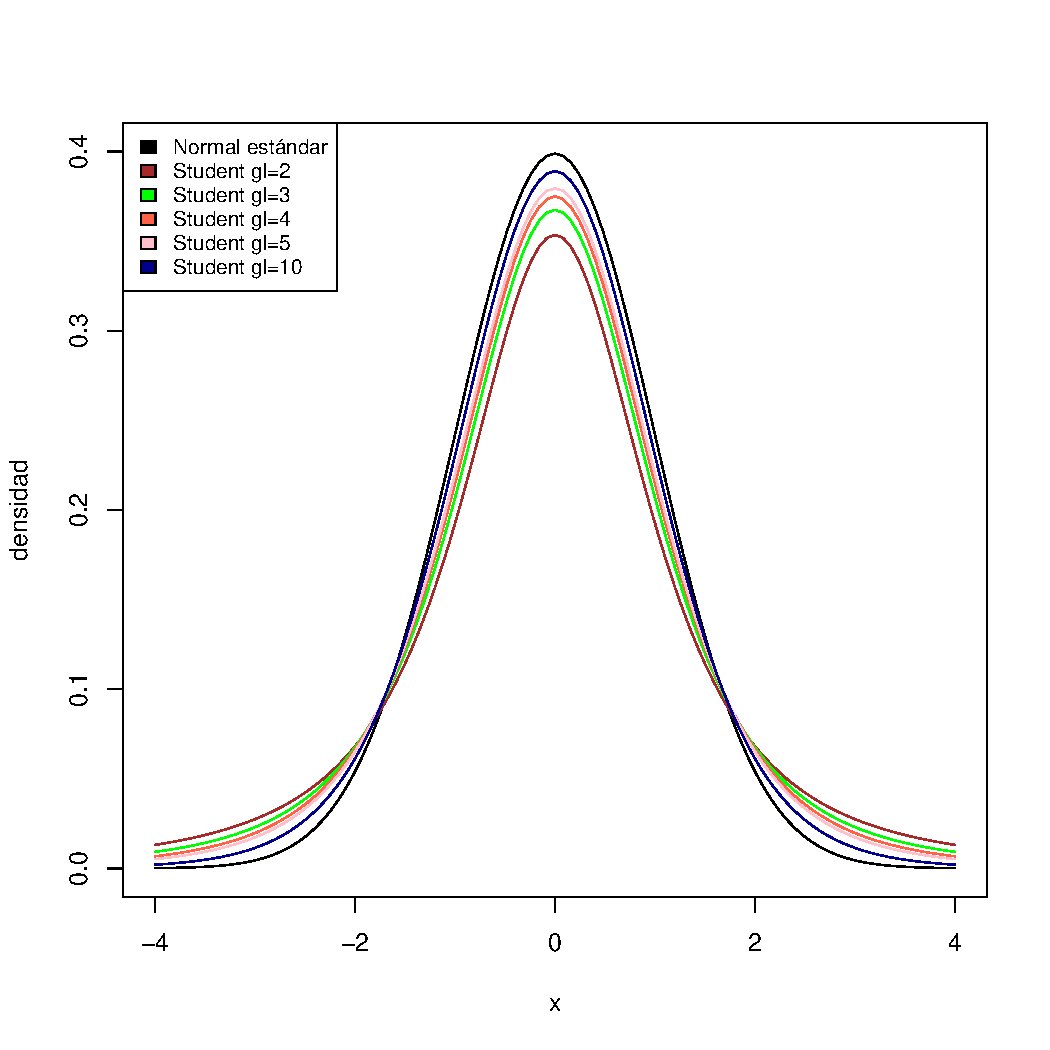
\includegraphics[width=\maxwidth]{figure/plotStudent-1} 

\end{knitrout}



\end{frame}



\begin{frame}
\frametitle{Distribución $t$ de Student}

Indicaremos con
\red{$t_{\nu,q}$} el  $q$-cuantil de una  v.a.  $X_{t_{\nu}}$ que sigue una distribución $t_\nu$:
$$
P(X_{t_{\nu}}\leq t_{\nu,q})=q
$$

Por simetría,
\red{$t_{\nu,q}=-t_{\nu,1-q}$}
\vspace*{-1ex}

\begin{center}
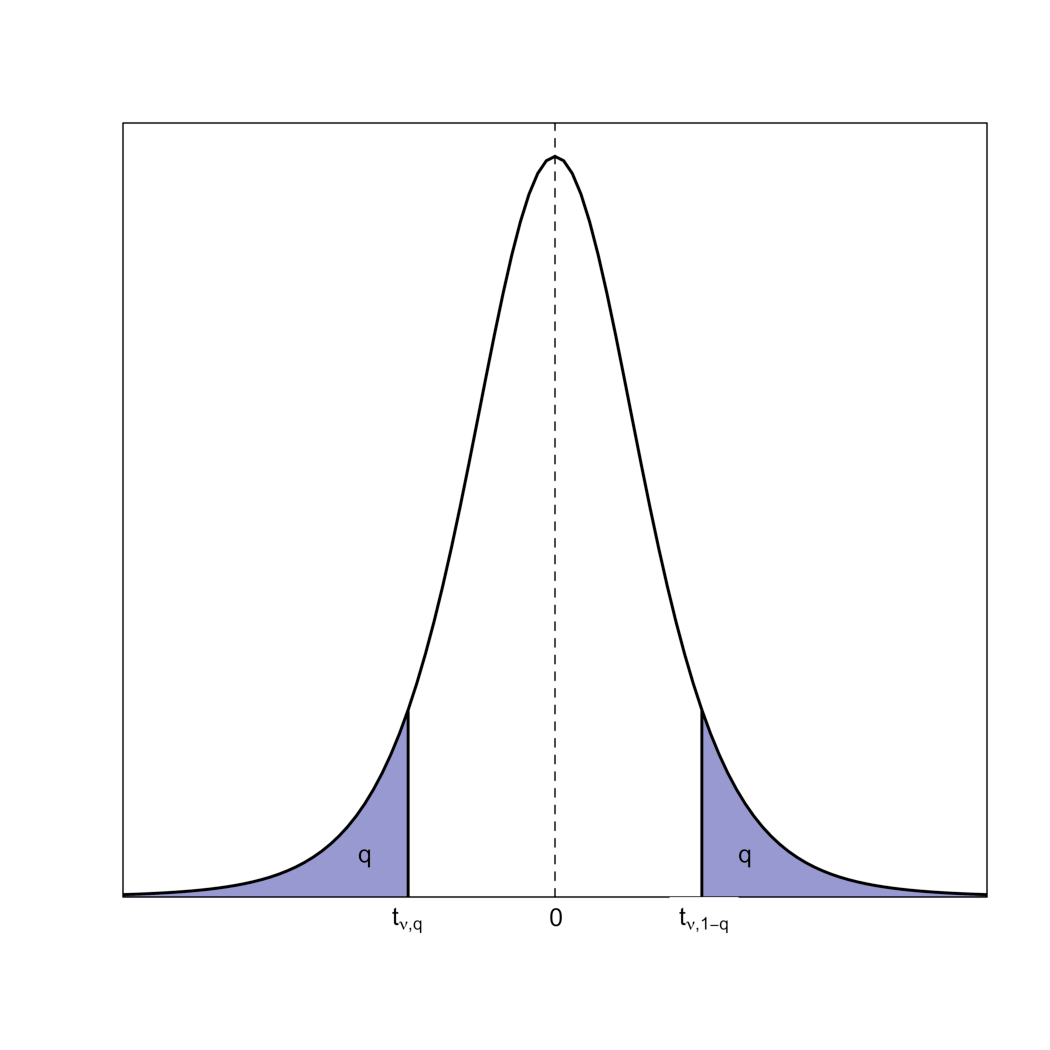
\includegraphics[width=0.6\linewidth]{quantilt}
\end{center}
\end{frame}



\begin{frame}
\frametitle{I.C. para $\mu$ de población normal con $\sigma$ desconocida}

Consideremos  la situación siguiente  :
\begin{itemize}
\item  $X$ una v.a.  normal con $\mu$ y $\sigma$ desconocidas

\item $X_1,\ldots,X_n$ una m.a.s. de $X$  de  tamaño  $n$, con media   $\overline{X}$ y varianza muestral $\widetilde{S}_X^2$
\end{itemize}


\begin{teorema}
En estas  condiciones, un intervalo  de confianza  del $(1-\alpha)\cdot 100\%$ I.C. para $\mu$ de una población normal con $\sigma$ conocida $\mu$
es 
$$
\left] 
\overline{X}-t_{n-1,1-\frac{\alpha}{2}} \frac{\widetilde{S}_{X}}{\sqrt{n}},
\overline{X}+t_{n-1,1-\frac{\alpha}{2}}\frac{\widetilde{S}_{X}}{\sqrt{n}} \right[
$$
\end{teorema}

\end{frame}

%
%
%\begin{frame}[fragile]
%\frametitle{$\mu$ de població normal con $\sigma$ desconocida}
%\vspace*{-5ex}
%
%\small
%\begin{verbatim}
%ICT=function(x,alpha){
%c(mean(x)-qt(1-alpha/2,length(x)-1)
%  *sd(x)/sqrt(length(x)),
%mean(x)+qt(1-alpha/2,length(x)-1)
%  *sd(x)/sqrt(length(x)))}
%set.seed(5)
%mu=1.5; sigma=0.4; alpha=0.05
%Poblacio=rnorm(10^6,mu,sigma)
%M=replicate(100,ICT(sample(Poblacio,15,replace=T),
%  alpha))
%plot(1:10,type="n",xlim=c(1.2,1.8),ylim=c(0,100),
%xlab="Valors",ylab="Replicacions")
%for(i in 1:100){color="grey";
%if((mu<M[1,i]) | (mu > M[2,i])){color = "red"}
%segments(M[1,i],i,M[2,i],i,col=color,lwd=3)}
%abline(v=mu,lwd=3)
%\end{verbatim}
%\end{frame}
%
%\begin{frame}
%\frametitle{$\mu$ de població normal con $\sigma$ desconocida}
%\vspace*{-1.2cm}
%
%\begin{center}
%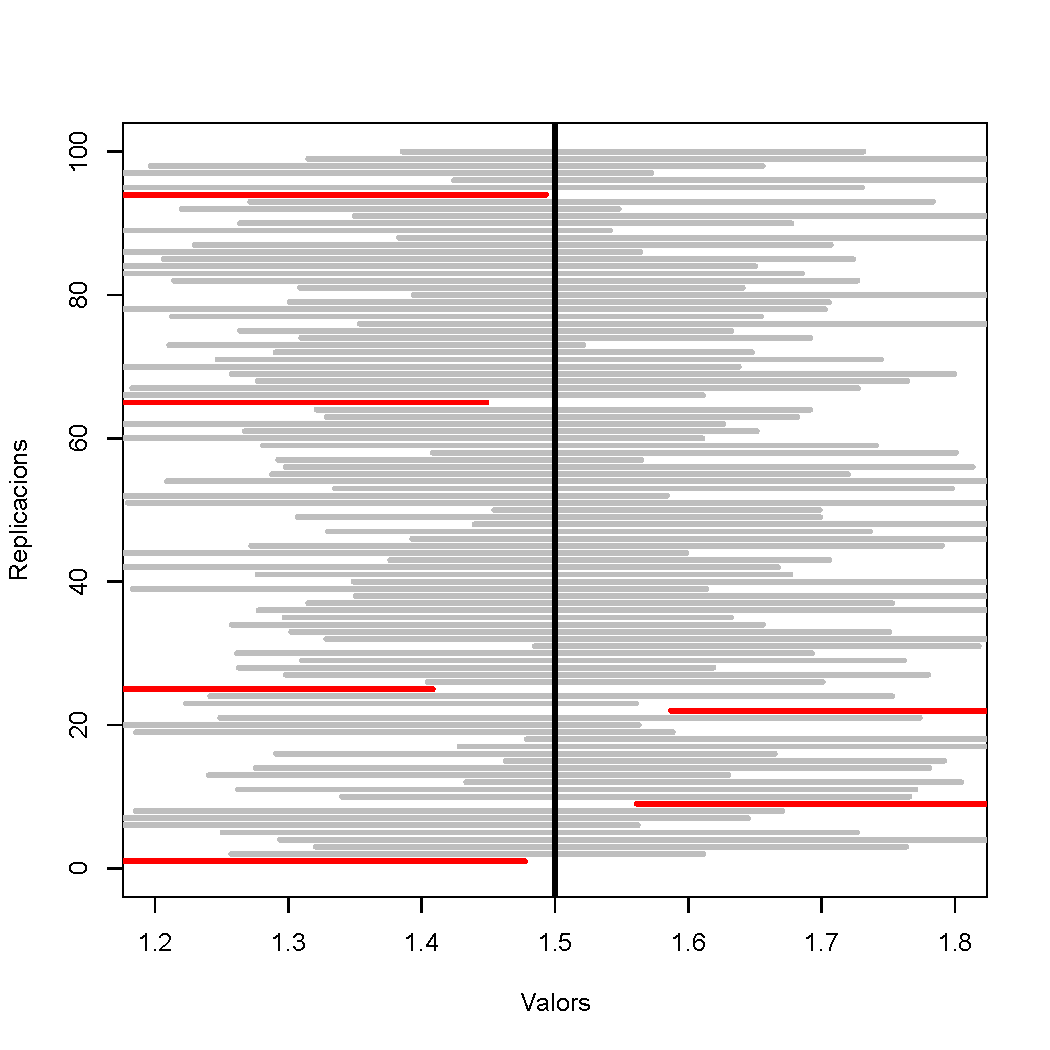
\includegraphics[width=0.9\linewidth]{intervals2}
%\end{center}
%\end{frame}
%
%
%
%




\begin{frame}
\frametitle{Ejemplo}

La empresa \textsl{3D-print} ofrece una impresora industrial de papel en color de alta capacidad. En su publicidad afirma que sus cartuchos imprimen una media de 500 mil copias con la especificación: 
\medskip

\blue{\texttt{Ficha técnica: Muestra de  tamaño  $n=100$,
población aproximadamente normal, nivel de confianza  del 90\%}}
\medskip 

La OCU (asociación de consumidores) desea comprobar estas  afirmaciones y su laboratorio toma una muestra aleatoria de  tamaño  $n=24$, obteniendo una media de $\overline{x}=518$ mil impresiones y una desviación típica muestral 
$\widetilde{s}=40$
\medskip

Con esta muestra ¿la media   poblacional anunciada por fabricante cae en el  intervalo de confianza  del 90\%?
\end{frame}

\begin{frame}[fragile]
\frametitle{Ejemplo}


\blue{Con esta muestra ¿la media   poblacional anunciada por fabricante cae en el  intervalo de confianza  del 90\%?}

Hay que  calcular el intervalo de confianza  para la $\mu$ de una población normal con $\sigma$ conocida $\mu$ con 
$$
n=24, \overline{x}=518, \widetilde{s}=40, \alpha=0.1
$$
Será
$$
\left] 
\overline{x}-t_{24,0.95} \frac{\widetilde{s}}{\sqrt{n}},
\overline{x}+t_{24,0.95} \frac{\widetilde{s}}{\sqrt{n}}\right[
$$
Consultando las tablas de la distribución  $t$ de Student, Obtenemos $t_{24,0.95}=1.71$
\end{frame}

\begin{frame}[fragile]
\frametitle{Ejemplo}

\blue{Con esta muestra ¿la media   poblacional anunciada por fabricante cae en el  intervalo de confianza  del 90\%?}

\begin{knitrout}\small
\definecolor{shadecolor}{rgb}{0.969, 0.969, 0.969}\color{fgcolor}\begin{kframe}
\begin{alltt}
\hlkwd{qt}\hlstd{(}\hlnum{0.95}\hlstd{,}\hlnum{24}\hlstd{)}
\end{alltt}
\begin{verbatim}
## [1] 1.710882
\end{verbatim}
\begin{alltt}
\hlkwd{round}\hlstd{(}\hlkwd{qt}\hlstd{(}\hlnum{0.95}\hlstd{,}\hlnum{24}\hlstd{),}\hlnum{2}\hlstd{)}
\end{alltt}
\begin{verbatim}
## [1] 1.71
\end{verbatim}
\end{kframe}
\end{knitrout}


Operando: $]531.962,504.038[$, y no contiene a 500 (¡pero se equivoca a favor del consumidor!)
\end{frame}



\begin{frame}
\frametitle{Observaciones }

\begin{itemize}
\item El intervalo de confianza  obtenido  está centrado   en $\overline{X}$
\medskip

\item La fórmula
$$
\left] 
\overline{X}-t_{n-1,1-\frac{\alpha}{2}} \frac{\widetilde{S}_{X}}{\sqrt{n}},
\overline{X}+t_{n-1,1-\frac{\alpha}{2}}\frac{\widetilde{S}_{X}}{\sqrt{n}} \right[
$$

nos da el I.C. para $\mu$ en una población normal con $\sigma$ conocida, el   intervalo de confianza  del $(1-\alpha)\cdot 100\%$ se  puede utilizar  cuando $X$ es normal y $n$ cualquiera
\bigskip

\item Si $n$ es grande $t_{n-1,1-\frac{\alpha}{2}}\approx z_{1-\frac{\alpha}{2}}$ y podemos \emph{aproximarlo}  mediante
$$
\left] 
\overline{X}-z_{1-\frac{\alpha}{2}} \frac{\widetilde{S}_{X}}{\sqrt{n}},
\overline{X}+z_{1-\frac{\alpha}{2}}\frac{\widetilde{S}_{X}}{\sqrt{n}} \right[
$$
\end{itemize}


\end{frame}







\subsection{I.C. para $\mu$ de una población normal con $\sigma$ conocida y  muestra grande}

\begin{frame}
\frametitle{I.C. para $\mu$ una población normal con $\sigma$ conocida y  muestra grande}

Consideremos la situación siguiente  :
\begin{itemize}
\item  $X$ una v.a.  \emph{cualquiera} con media   poblacional $\mu$ desconocida y desv. típ. $\sigma$ conocida

\item $X_1,\ldots,X_n$ una m.a.s. de $X$, con media   $\overline{X}$

\item \emph{$n$ es grande} (pongamos que $n\geq 40$)
\end{itemize}

%\only<2>{En estas  condiciones (T.C.L.)

En estas  condiciones (T.C.L.)
$$
\frac{\overline{X}-\mu}{\frac{\sigma}{\sqrt{n}}}\approx N(0,1)
$$


\begin{teorema}
En estas  condiciones, podemos tomar como intervalo  de confianza  del $(1-\alpha)\cdot 100\%$ I.C. para $\mu$ de población normal con $\sigma$ conocida $\mu$
$$
\left]\overline{X}-z_{1-\frac{\alpha}{2}}\frac{\sigma}{\sqrt{n}},
    \overline{X}+z_{1-\frac{\alpha}{2}}\frac{\sigma}{\sqrt{n}}\right[
$$
\end{teorema}
\end{frame}


\begin{frame}
\frametitle{I.C. para $\mu$ de población normal con $\sigma$ conocida muestra grande}

Consideremos  la situación siguiente  :
\begin{itemize}
\item  $X$ una v.a.  \emph{cualquiera} con media   poblacional $\mu$ desconocida  \emph{y desv. típ. $\sigma$ desconocida}

\item $X_1,\ldots,X_n$ una m.a.s. de $X$, con media   $\overline{X}$ \emph{y desviación típica muestral $\widetilde{S}_X$}

\item \emph{$n$ es grande} (pongamos que $n\geq 40$)
\end{itemize}
%\pause


\begin{block}{``Teorema''}
En estas  condiciones, se recomienda tomar como  intervalo  de
confianza  del $(1-\alpha)\cdot 100\%$  para $\mu$ de población normal con $\sigma$ conocida $\mu$
$$
\left]\overline{X}-z_{1-\frac{\alpha}{2}}\frac{\widetilde{S}_X}{\sqrt{n}},
    \overline{X}+z_{1-\frac{\alpha}{2}}\frac{\widetilde{S}_X}{\sqrt{n}}\right[
$$
\end{block}



\end{frame}

%
%\begin{frame}[fragile]
%\frametitle{$\mu$ I.C. para $\mu$ de población normal con $\sigma$ conocidamostres grans}
%\vspace*{-2ex}
%
%\small
%\begin{verbatim}
%ICZ2=function(x,alpha){
%  c(mean(x)-qnorm(1-alpha/2)*sd(x)/sqrt(length(x)), 
%  mean(x)+qnorm(1-alpha/2)*sd(x)/sqrt(length(x)))
%}
%set.seed(15)
%lconda=1.5; alpha=0.05
%Poblacio=rpois(10^6,lconda)
%M=replicate(100,ICZ(sample(Poblacio,40,replace=T),
%  alpha))
%plot(1:10,lwd=3,xlim=c(1.2,1.8),ylim=c(0,100),
%xlab="Valors",ylab="Replicacions")
%for(i in 1:100){
%  color="grey";
%  if((mu<M[1,i]) | (mu > M[2,i])){color = "red"}
%  segments(M[1,i],i,M[2,i],i,col=color,lwd=3)
%}
%abline(v=mu,lwd=3)
%\end{verbatim}
%\end{frame}
%
%\begin{frame}
%\frametitle{$\mu$ I.C. para $\mu$ de población normal con $\sigma$ conocidamostres grans}
%\vspace*{-1.2cm}
%
%\begin{center}
%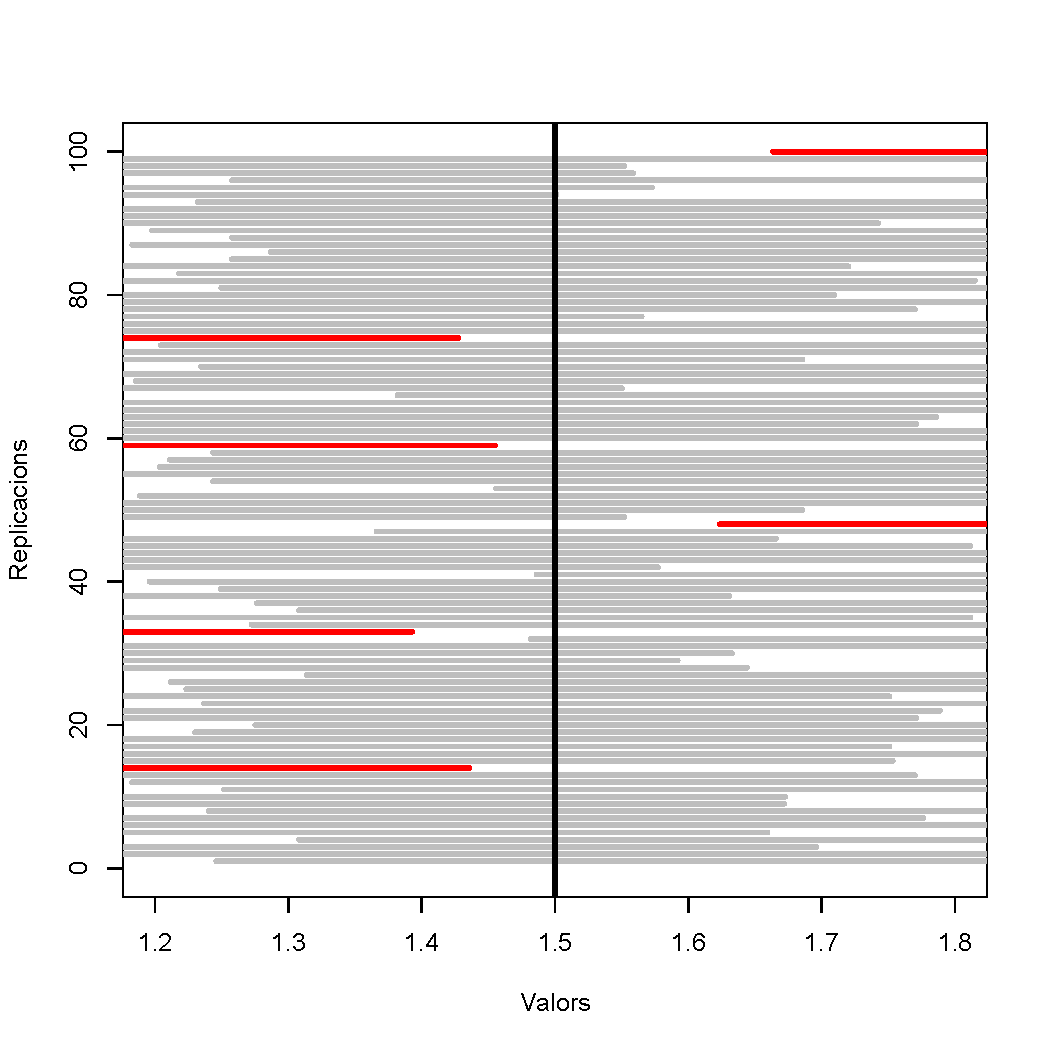
\includegraphics[width=0.9\linewidth]{intervals3}
%\end{center}
%\end{frame}
%


\begin{frame}[fragile]
\frametitle{Ejemplo}
\vspace*{-2ex}
Consultad el enlace \MYhref[green]{https://twitter.com/guardiacivil/status/805154653977608192/photo/1}{Guardia civil informa...}

Simulemos un experimento en el que se ha medido la tasa oficial  de  alcoholemia en sangre a 40 varones (sobrios) después de tomar 3 cañas de cerveza de 330 ml.
El siguiente código simula este experimento supuesto que la tasa de alcoholemia siga una distribución normal de media 0.7 (supuestamente desconocida) y desviación típica 0.1 (supuestamente desconocida)



\begin{knitrout}\scriptsize
\definecolor{shadecolor}{rgb}{0.969, 0.969, 0.969}\color{fgcolor}\begin{kframe}
\begin{alltt}
\hlkwd{set.seed}\hlstd{(}\hlnum{1234}\hlstd{)}\hlcom{# por reproducibilidad}
\hlstd{tasa_alcoholemia}\hlkwb{=}\hlkwd{round}\hlstd{(}\hlkwd{rnorm}\hlstd{(}\hlnum{40}\hlstd{,}\hlkwc{mean}\hlstd{=}\hlnum{0.7}\hlstd{,}\hlkwc{sd}\hlstd{=}\hlnum{0.1}\hlstd{),}\hlnum{2}\hlstd{)}
\hlkwd{head}\hlstd{(tasa_alcoholemia,}\hlnum{10}\hlstd{)}
\end{alltt}
\begin{verbatim}
##  [1] 0.58 0.73 0.81 0.47 0.74 0.75 0.64 0.65 0.64 0.61
\end{verbatim}
\end{kframe}
\end{knitrout}
\end{frame}

\begin{frame}[fragile]
\frametitle{Ejemplo}
\vspace*{-2ex}

\begin{knitrout}\scriptsize
\definecolor{shadecolor}{rgb}{0.969, 0.969, 0.969}\color{fgcolor}\begin{kframe}
\begin{alltt}
\hlstd{media}\hlkwb{=}\hlkwd{round}\hlstd{(}\hlkwd{mean}\hlstd{(tasa_alcoholemia),}\hlnum{3}\hlstd{)}
\hlstd{media}
\end{alltt}
\begin{verbatim}
## [1] 0.659
\end{verbatim}
\begin{alltt}
\hlstd{des.tip}\hlkwb{=}\hlkwd{round}\hlstd{(}\hlkwd{sd}\hlstd{(tasa_alcoholemia),}\hlnum{3}\hlstd{)}
\hlstd{des.tip}
\end{alltt}
\begin{verbatim}
## [1] 0.091
\end{verbatim}
\end{kframe}
\end{knitrout}
Así que tenemos los siguientes estadísticos
$$
\overline{x}=0.659,\quad \widetilde{s}=0.091
$$

%\pause

\end{frame}


\begin{frame}
\frametitle{Ejemplo}
\blue{Calculad  un intervalo del que podamos afirmar que con una probabilidad del 95\% contiene la media poblacional de  la tasa de alcoholemia  para hombres después de beber 3 cerveza de 330ml.}
\medskip

Nos piden un \emph{intervalo de confianza  del 95\%}  para $\mu$ de una población normal con $\sigma$ conocida  de la v.a. $X$ ``tasa de alcoholemia  para hombres después de beber 3 cervezas de 330ml''

No conocemos la distribución de  $X$, pero $n=40$ es "grande"
\end{frame}

\begin{frame}
\frametitle{Ejemplo}
Podemos emplear
\red{$$
\left]\overline{x}-z_{1-\frac{\alpha}{2}}\frac{\widetilde{s}}{\sqrt{n}},
    \overline{x}+z_{1-\frac{\alpha}{2}}\frac{\widetilde{s}}{\sqrt{n}}\right[
$$}
donde
$$
\begin{array}{c}
n=40,\overline{x}=0.659,\widetilde{s}=0.091,\\[1ex]
\alpha=0.05\Rightarrow z_{1-\frac{\alpha}{2}}=z_{0.975}=1.96
\end{array}
$$
%\pause
$$
]0.631, 0.687[
$$

Podemos afirmar con un 95\% de confianza  que la tasa de alcoholemia media en sangre de la población de hombres después de  beber  3  cervezas de 330ml está entre 
0.631 y 
0.687

\end{frame}



\begin{frame}
\frametitle{Ejemplo}
\vspace*{-2ex}

Se ha tomado una muestra del tiempo de visualización de vídeo semanal en horas de  1000  usuarios de un canal de videos por internet. Se ha obtenido  una media   muestral de 9.5 horas/semana con una desviació típica muestral de 0.5 horas/semana. 
\medskip

\blue{Calculad un intervalo de confianza  del 95\% para la media poblacional del número de horas visualizadas por semana supuesto que sigue aproximadamente una población normal con  $\sigma$ desconocida}

\end{frame}


\begin{frame}[fragile]
\frametitle{Ejemplo}
\vspace*{-2ex}

Como $n=1000$ es grande, podemos utilizar

\red{$$
\left]\overline{x}-z_{1-\frac{\alpha}{2}}\frac{\widetilde{s}}{\sqrt{n}},
    \overline{x}+z_{1-\frac{\alpha}{2}}\frac{\widetilde{s}}{\sqrt{n}}\right[
$$}
donde
$$
\overline{x}=9.5,\ \widetilde{s}=0.5,\
\alpha=0.05,\  z_{1-\frac{\alpha}{2}}=z_{0.975}=1.96
$$
Con estos valores obtenemos que 

\begin{knitrout}\small
\definecolor{shadecolor}{rgb}{0.969, 0.969, 0.969}\color{fgcolor}\begin{kframe}
\begin{alltt}
\hlstd{media}\hlkwb{=}\hlnum{9.5}
\hlstd{sd}\hlkwb{=}\hlnum{0.5}
\hlstd{n}\hlkwb{=}\hlnum{1000}
\hlstd{alpha}\hlkwb{=}\hlnum{0.5}
\end{alltt}
\end{kframe}
\end{knitrout}
\end{frame}

\begin{frame}[fragile]
\frametitle{Ejemplo}
\begin{knitrout}
\definecolor{shadecolor}{rgb}{0.969, 0.969, 0.969}\color{fgcolor}\begin{kframe}
\begin{alltt}
\hlstd{cuantil}\hlkwb{=}\hlkwd{qnorm}\hlstd{(}\hlnum{1}\hlopt{-}\hlnum{0.5}\hlopt{/}\hlnum{2}\hlstd{)}
\hlstd{cuantil}
\end{alltt}
\begin{verbatim}
## [1] 0.6744898
\end{verbatim}
\begin{alltt}
\hlstd{a}\hlkwb{=}\hlkwd{round}\hlstd{(media}\hlopt{-}\hlstd{cuantil}\hlopt{*}\hlstd{sd}\hlopt{/}\hlkwd{sqrt}\hlstd{(n),}\hlnum{3}\hlstd{)}
\hlstd{a}
\end{alltt}
\begin{verbatim}
## [1] 9.489
\end{verbatim}
\begin{alltt}
\hlstd{b}\hlkwb{=}\hlkwd{round}\hlstd{(media}\hlopt{+}\hlstd{cuantil}\hlopt{*}\hlstd{sd}\hlopt{/}\hlkwd{sqrt}\hlstd{(n),}\hlnum{3}\hlstd{)}
\hlstd{b}
\end{alltt}
\begin{verbatim}
## [1] 9.511
\end{verbatim}
\end{kframe}
\end{knitrout}



Por lo tanto 

$$
]9.489,9.511[
%]9.47, 9.53[
$$

Podemos afirmar con un 95\% de confianza  que la media poblacional de  vídeo consumido en horas por semana está entre $9.47$  y  $9.53$ horas/semana


\end{frame}



\begin{frame}
\frametitle{Amplitud}
\vspace*{-2ex}

La amplitud de 
$$
\left]\overline{X}-z_{1-\frac{\alpha}{2}}\frac{\widetilde{S}_X}{\sqrt{n}},
    \overline{X}+z_{1-\frac{\alpha}{2}}\frac{\widetilde{S}_X}{\sqrt{n}}\right[
$$
es
$$
A=2z_{1-\frac{\alpha}{2}}\frac{\widetilde{S}_X}{\sqrt{n}}
$$
Para determinar $n$ (grande) que dé cómo  máximo una amplitud $A$ prefijada, necesitamos $\widetilde{S}_X$, que depende de la muestra.
\medskip

 Soluciones:
\begin{itemize}
\item Si sabemos  la desv. típ. poblacional $\sigma$, la utilizaremos en lugar de  $\widetilde{S}_X$
\item Si hemos tomado una muestra previa (\emph{piloto}), emplearemos  la desviación típica muestral para estimar $\sigma$
\end{itemize}
\end{frame}



\begin{frame}
\frametitle{Amplitud}

\begin{block}{}
De una población $X$ hemos tomado una  \emph{m.a.s.\ piloto} que ha tenido una  desviación típica muestral $\widetilde{s}_{pilot}$.
\medskip

Estimaremos que el tamaño  mínima $n$ de una m.a.s.\ de $X$ que dé un intervalo de confianza  I.C. para $\mu$ de una población normal
con $\sigma$ desconocida de nivell de confianza  $1-\alpha$ y amplitud máxima $A_0$ es 
$$
n=\left\lceil \Big(2z_{1-\frac{\alpha}{2}}\frac{\widetilde{s}_{pilot}}{A_0}\Big)^2\right\rceil
$$
\end{block}



\end{frame}





\begin{frame}
\frametitle{Ejemplo}

Queremos  estimar la estatura media de los  estudiantes de la UIB. Queremos obtener un intervalo de confianza  del 99\% con 
una precisión máxima de 1 cm. En una muestra piloto de 25 estudiantes,  obtuvimos que  
$$
\overline{x} = 170\mbox{ cm}, \widetilde{s}=10\mbox{ cm}
$$

¿Basándonos en estos  datos, cuál es el tamaño necesario  de la muestra para poder alcanzar nuestro objetivo?

\end{frame}


\begin{frame}
\frametitle{Ejemplo}

$$
n=
\left\lceil \Big(2z_{1-\frac{\alpha}{2}}\frac{\widetilde{s}_{pilot}}{A}\Big)^2\right\rceil=
\left\lceil \Big(z_{1-\frac{\alpha}{2}}\frac{\widetilde{s}_{pilot}}{A/2}\Big)^2\right\rceil
$$

\begin{itemize}
\item Precisión = error máximo = ${A}/{2}=1$
\medskip

\item $\widetilde{s}_{pilot}=10$
\medskip

\item $\alpha=0.01\Rightarrow z_{1-\frac{\alpha}{2}}=z_{0.995}=2.58$
\end{itemize}
Dóna
$$
n=\left\lceil \Big(2.58\cdot \frac{10}{1}\Big)^2\right\rceil=\lceil 665.64\rceil=666
$$

\end{frame}



\subsection{I.C para una proporción }


\begin{frame}
\frametitle{I.C para una proporción}

Consideremos la situación siguiente  :
\begin{itemize}
\item  $X$ una v.a. Bernoulli con $p$ desconocida

\item $X_1,\ldots,X_n$ una m.a.s. de $X$, con número de éxitos  $x$ y por lo tanto la frecuencia relativa de éxitos  es $\widehat{p}_{X}=x/n$
\end{itemize}

Recordad que $X$ es $B(n,p)$
\scriptsize{
\begin{block}{Método ``exacto'' o de Clopper-Pearson}
Un intervalo de confianza  $]p_0,p_1[$ del $(1-\alpha)100\%$nivel de confianza para $p$ de una población se obtiene encontrando el $p_0$ más grande y el $p_1$ más pequeño tales que
$$
\displaystyle\sum_{k=x}^n 
\left(\begin{array}{c} n \\ k\end{array}\right)
\cdot p_0^k\cdot (1-p_0)^{n-k}\leq \frac{\alpha}{2},\quad
\displaystyle\sum_{k=0}^x \left(\begin{array}{c} n \\ k\end{array}\right)\cdot p_1^k\cdot(1-p_1)^{n-k}\leq \frac{\alpha}{2}
$$
\end{block}
Manualmente (consultando las tablas) sería un trabajo muy pesado.
}
\end{frame}

%\end{document}

\begin{frame}[fragile]
\frametitle{I.C.\ para  una proporción}
\vspace*{-2ex}

El paquete \texttt{epitools} incorpora la función 
\begin{center}
{\tt binom.exact(éxitos, tamaño ,conf.)}
\end{center}
para calcularlo
\medskip

\blue{De 10 pacientes tratados con un medicamento, 2 se han curado. Dar un intervalo de confianza  del 95\% I.C. 
para  la proporción poblacional $p$ de pacientes que este medicamento sana}

\begin{knitrout}\scriptsize
\definecolor{shadecolor}{rgb}{0.969, 0.969, 0.969}\color{fgcolor}\begin{kframe}
\begin{alltt}
\hlcom{#descomentar para instalar}
\hlcom{#install.packages("epitools",dep=TRUE)}
\hlkwd{library}\hlstd{(epitools)}
\hlstd{solución}\hlkwb{=}\hlkwd{round}\hlstd{(}\hlkwd{binom.exact}\hlstd{(}\hlnum{2}\hlstd{,}\hlnum{10}\hlstd{,}\hlnum{0.95}\hlstd{),}\hlnum{3}\hlstd{)}
\hlstd{solución}
\end{alltt}
\begin{verbatim}
##   x  n proportion lower upper conf.level
## 1 2 10        0.2 0.025 0.556       0.95
\end{verbatim}
\end{kframe}
\end{knitrout}

Da $]0.025,0.556[$
\end{frame}

\subsection{I.C. para la proporción poblacional muestras grandes}


\begin{frame}
\frametitle{I.C. para la proporción poblacional muestras grandes I}

Consideremos la situación siguiente  :
\begin{itemize}
\item  $X$ una v.a. Bernoulli con $p$ desconocida

\item $X_1,\ldots,X_n$ una m.a.s. de $X$, con $n$  gran (por Ejemplo, $n\geq 40$) y frecuencia relativa de éxitos $\widehat{p}_{X}$
\end{itemize}
\medskip

En estas  condiciones (por el  T.C.L.), 
$$
Z=\dfrac{\widehat{p}_{X}-p}
{\sqrt{\frac{p(1-p)}{n}}}\approx N(0,1)
$$
\end{frame}


\begin{frame}
\frametitle{I.C. para la proporción $p$ muestral muestras grandes I}
Por lo tanto

$$
P\left(-z_{1-\frac{\alpha}{2}}\leq \dfrac{\widehat{p}_{X}-p}
{\sqrt{\frac{p(1-p)}{n}}}\leq z_{1-\frac{\alpha}{2}}\right)=1-\alpha
$$

El problema es que no conocemos $p$, la literatura plantea entre otras soluciones :

\begin{itemize}
\item[I)] El método de Wilson
\item[II)] La solución de Laplace (1812)
\end{itemize}

Exponemos estas soluciones a continuación
\end{frame}


\begin{frame}
\frametitle{I.C. para la proporción poblacional muestras grandes I}

\begin{block}{Método de Wilson}
En estas  condiciones, un intervalo  de confianza  del $(1-\alpha)\cdot 100\%$ I.C. para $p$ es  (donde $\widehat{q}_{X}=1-\widehat{p}_{X}$)
$$
\begin{array}{l}
\displaystyle \left]\frac{\widehat{p}_{X}+\frac{z_{1-{\alpha}/{2}}^2}{2n}-z_{1-{\alpha}/{2}}\sqrt{\frac{\widehat{p}_{X}\widehat{q}_{X}}{n}+\frac{z_{1-{\alpha}/{2}}^2}{4n^2}}}{1+\frac{z_{1-{\alpha}/{2}}^2}{n}}\right.,\\[2ex]
\hspace*{2cm} \displaystyle \left.\frac{\widehat{p}_{X}+\frac{z_{1-{\alpha}/{2}}^2}{2n}+z_{1-{\alpha}/{2}}\sqrt{\frac{\widehat{p}_{X}\widehat{q}_{X}}{n}+\frac{z_{1-{\alpha}/{2}}^2}{4n^2}}}{1+\frac{z_{1-{\alpha}/{2}}^2}{n}}\right[
\end{array}
$$
\end{block}
\medskip

\texttt{binom.wilson} del paquete \texttt{epitools}
\end{frame}



\begin{frame}[fragile]
\frametitle{I.C. para la proporción poblacional muestras grandes II}

\begin{itemize}
\item  $X$ una v.a. Bernoulli con $p$ desconocida
\item $X_1,\ldots,X_n$ una m.a.s. de $X$, con $n$  grande y $\widehat{p}_{X}$ alejado  de 0 y 1. Por ejemplo, tal que:
$$
n\geq 100, n\widehat{p}_{X}\geq 10,  n(1-\widehat{p}_{X})\geq 10
$$
\end{itemize}
\medskip

\begin{block}{Fórmula de Laplace (1812)}
Bajo  estas  condiciones, se puede tomar como intervalo de  confianza  del $(1-\alpha)\cdot 100\%$ para $p$
$$
\left]\widehat{p}_{X}-z_{1-\frac{\alpha}{2}}\sqrt{\frac{\widehat{p}_{X}
(1-\widehat{p}_{X})}{n}},
\widehat{p}_{X}+z_{1-\frac{\alpha}{2}}\sqrt{\frac{\widehat{p}_{X}
(1-\widehat{p}_{X})}{n}}\right[$$
\end{block}
\end{frame}



\begin{frame}
\frametitle{Ejemplo}

En una muestra aleatoria de 500 familias con niños en edad escolar se encontró que 
340 introducían fruta de forma diaria en la dieta de sus hijos
\medskip

Calculad un intervalo de confianza  del 95\% para  conocida la proporción real de
familias de esta ciudad con niños en edad escolar que incorporen fruta fresca de
forma diaria en la dieta de sus hijos.


\end{frame}
\begin{frame}
\frametitle{Ejemplo}

$X=$ ``Aportan diariamente fruta a la dieta de sus hijos''\\
 es $Be(p)$, y buscamos el  intervalo de confianza  del 95\%  para $p$ 
\bigskip

Como que $n=500\geq 100$, $n\widehat{p}_X=340\geq 10$ y $n\cdot (1-\widehat{p}_X)=160\geq 10$, podemos utilizar  este intervalo
$$
\left]\widehat{p}_{X}-z_{1-\frac{\alpha}{2}}\sqrt{\frac{\widehat{p}_{X}
(1-\widehat{p}_{X})}{n}},
\widehat{p}_{X}+z_{1-\frac{\alpha}{2}}\sqrt{\frac{\widehat{p}_{X}
(1-\widehat{p}_{X})}{n}}\right[
$$
con
$$
n=500, \widehat{p}_{X}=\dfrac{340}{500}=0.68
$$
Que vale (recordad que  {\small $\alpha=0.05\Rightarrow z_{1-\frac{\alpha}{2}}=z_{0.975}=1.96$})
$$
\red{]0.639,0.721[}
$$

\end{frame}

\begin{frame}[fragile]
\frametitle{Ejemplo}

Con los otros métodos:


\begin{knitrout}
\definecolor{shadecolor}{rgb}{0.969, 0.969, 0.969}\color{fgcolor}\begin{kframe}
\begin{alltt}
\hlkwd{round}\hlstd{(}\hlkwd{binom.exact}\hlstd{(}\hlnum{340}\hlstd{,}\hlnum{500}\hlstd{,}\hlnum{0.95}\hlstd{),}\hlnum{3}\hlstd{)}
\end{alltt}
\begin{verbatim}
##     x   n proportion lower upper conf.level
## 1 340 500       0.68 0.637 0.721       0.95
\end{verbatim}
\begin{alltt}
\hlkwd{round}\hlstd{(}\hlkwd{binom.wilson}\hlstd{(}\hlnum{340}\hlstd{,}\hlnum{500}\hlstd{,}\hlnum{0.95}\hlstd{),}\hlnum{3}\hlstd{)}
\end{alltt}
\begin{verbatim}
##     x   n proportion lower upper conf.level
## 1 340 500       0.68 0.638 0.719       0.95
\end{verbatim}
\end{kframe}
\end{knitrout}


Obtenemos:
\medskip

\begin{itemize}
\item Clopper-Pearson: $]0.637,0.721[$
\medskip

\item Wilson: $]0.638, 0.719[$
\medskip

\item Laplace: $]0.639,0.721[$
\end{itemize}

\end{frame}

\begin{frame}
\frametitle{Ejemplo}

\blue{En un ensayo de un nuevo  tratamiento de quimioterapia, en una muestra de $n$ (grande) enfermos tratados, ninguno desarrolla cáncer testicular
como  efecto secundario. Calculad un intervalo de confianza  al 95\%  para la proporción poblacional  de enfermos tratados con esta
quimioterapia que no tienen cáncer testicular.}
%\pause
\bigskip

No podemos emplear la fórmula de Laplace, porqué $\widehat{p}_X=0$. Tenemos que emplear el método de Wilson:


\end{frame}

\begin{frame}
\frametitle{Ejemplo}
\vspace*{-5ex}

{\small
$$
\begin{array}{l}
\displaystyle \left]\frac{\widehat{p}_{X}+\frac{z_{1-{\alpha}/{2}}^2}{2n}-z_{1-{\alpha}/{2}}\sqrt{\frac{\widehat{p}_{X}\widehat{q}_{X}}{n}+\frac{z_{1-{\alpha}/{2}}^2}{4n^2}}}{1+\frac{z_{1-{\alpha}/{2}}^2}{n}}\right.,\\[2ex]
\hspace*{2cm} \displaystyle \left.\frac{\widehat{p}_{X}+\frac{z_{1-{\alpha}/{2}}^2}{2n}+z_{1-{\alpha}/{2}}\sqrt{\frac{\widehat{p}_{X}\widehat{q}_{X}}{n}+\frac{z_{1-{\alpha}/{2}}^2}{4n^2}}}{1+\frac{z_{1-{\alpha}/{2}}^2}{n}}\right[
\end{array}
$$
%\pause
$$
\left]\frac{\frac{1.96^2}{2n}- 1.96\sqrt{\frac{1.96^2}{4n^2}}}{1+\frac{1.96^2}{n}},
\frac{\frac{1.96^2}{2n}+ 1.96\sqrt{\frac{1.96^2}{4n^2}}}{1+\frac{1.96^2}{n}}\right[
=\Big]0,\frac{1.96^2}{n+1.96^2}\Big[
$$

}

\red{En el área de sanidad se emplea  $\Big]0,\dfrac{3}{n}\Big[$ (la regla del 3)}


\end{frame}


\begin{frame}
\frametitle{Observaciones }
\begin{itemize}
\item El método  de Wilson da un I.C. centrado   en
$$
\frac{\widehat{p}_{X}+\frac{z_{1-{\alpha}/{2}}^2}{2n}}{1+\frac{z_{1-{\alpha}/{2}}^2}{n}}
=\frac{2n\widehat{p}_{X}+ z_{1-\frac{\alpha}{2}}^2}{2n+2 z_{1-\frac{\alpha}{2}}^2}
$$

\item No se conoce una fórmula para el centro del I.C. de Clopper-Pearson.

\item La fórmula de Laplace dóna un I.C.  centrado   en $\widehat{p}_{X}$
\medskip

\item Cuando $n$ crece se reduce la amplitud del intervalo de confianza 

\end{itemize}

\end{frame}


\begin{frame}
\frametitle{Amplitud}

La amplitud del intervalo de confianza  de Laplace es 
$$
A=2 z_{1-\frac{\alpha}{2}} \sqrt{\frac{\widehat{p}_{X} (1-\widehat{p}_{X})}{n}}
$$
No podem determinar el   tamaño  de la mostra para que el intervalo de confianza  tenga una cierta amplitud máxima sin
conocer $\widehat{p}_{X}$, que obviamente no conocemos sin hacer una muestra

\end{frame}

\begin{frame}
\frametitle{Amplitud}
\vspace*{-4ex}

$$
A=2 z_{1-\frac{\alpha}{2}} \sqrt{\frac{\widehat{p}_{X} (1-\widehat{p}_{X})}{n}}
$$
El máximo de $\sqrt{\widehat{p}_{X} (1-\widehat{p}_{X})}$ se alcanza en  $\widehat{p}_{X}=0.5$ 
\only<1>{
\begin{center}
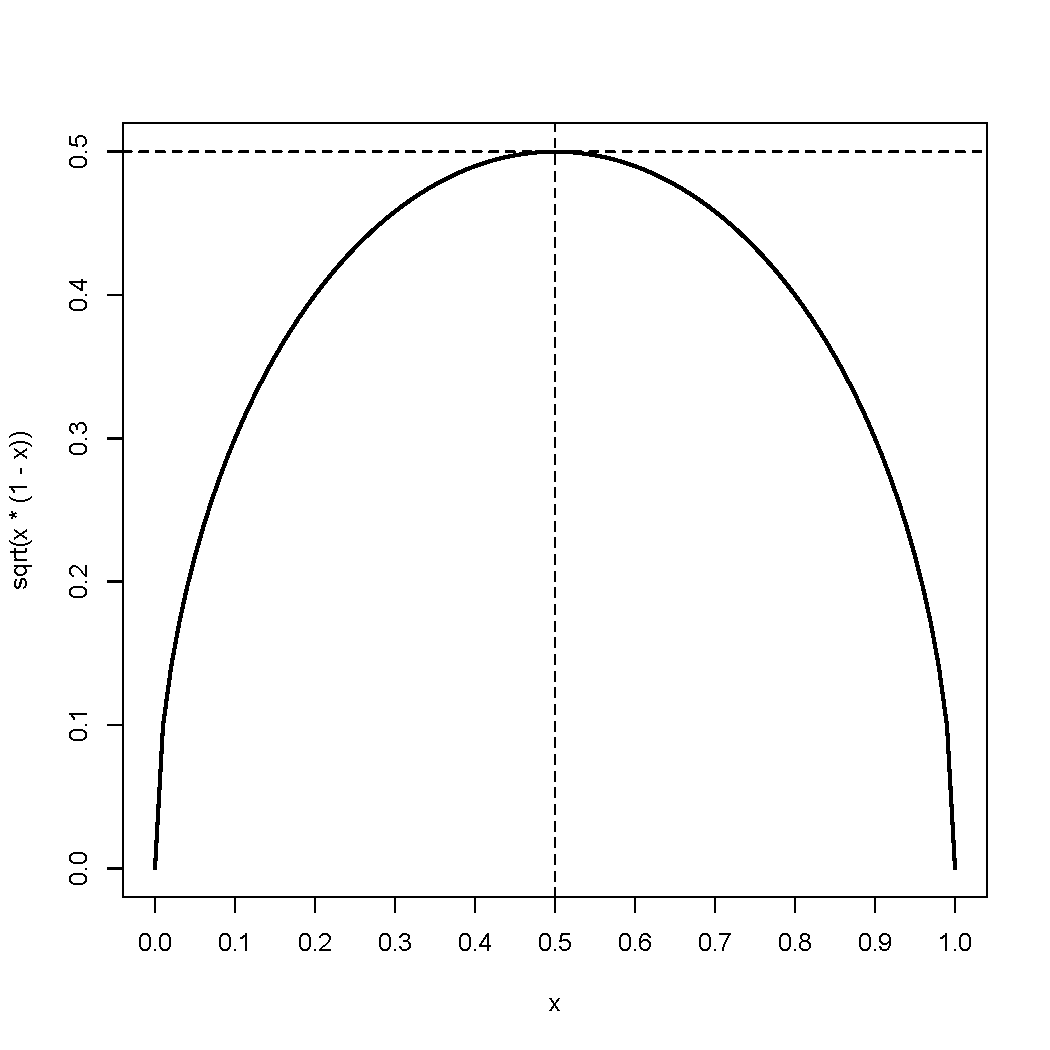
\includegraphics[width=0.6\linewidth]{p(1-p).pdf}
\end{center}}

\only<2>{\vspace*{5ex}

Por lo tanto, calcularemos $n$ para obtener una  amplitud máxima $A_0$ suponiendo el peor de los casos ($\widehat{p}_{X}=0.5$):
$$
A_0\geq 2z_{1-\frac{\alpha}{2}}\sqrt{\frac{0.5^2}{n}}=\frac{z_{1-\frac{\alpha}{2}}}{\sqrt{n}}
\Rightarrow
\red{n=\left\lceil\frac{z_{1-\frac{\alpha}{2}}^2}{A_0^2}\right\rceil}
$$}

\end{frame}


\begin{frame}
\frametitle{Ejemplos}

\begin{center}
\hspace*{-0.5cm}

\includegraphics[width=1.1\linewidth]{plagiUIB1.jpg}\bigskip

\hspace*{-0.5cm}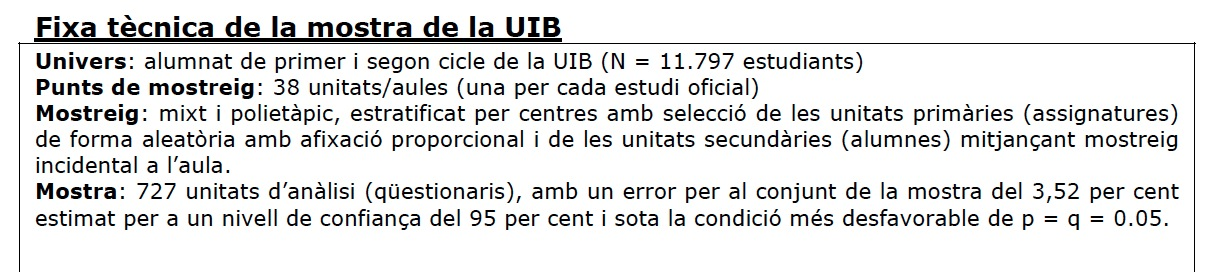
\includegraphics[width=1.1\linewidth]{plagiUIB2.jpg}
\end{center}
$$
\mbox{Error}=
%\pause
\frac{1.96\cdot 0.5}{\sqrt{727}}\approx 0.0363
$$
\end{frame}



\begin{frame}
\frametitle{Ejemplo}
Quemos estudiar qué fración teléfonos móviles utilizan android. Para determinar esta proporción con un  nivel de confianza  del 95\%
y garantizar un error máximo de 0.05, ¿de qué  tamaño  ha de ser la muestra \emph{en el peor de los casos}?
$$
n=\left\lceil\frac{z_{1-\frac{\alpha}{2}}^2}{A^2}\right\rceil
$$
on
$$
\frac{A}{2}=0.05,\quad z_{1-\frac{\alpha}{2}}=z_{0.975}=1.96
$$
Obtenemos que  $n= \lceil 384.16\rceil=385$.

\end{frame}




%\subsection{$\sigma$ de població normal}
\subsection{I.C. para $\sigma^2$ de una población normal}

\begin{frame}
\frametitle{I.C. de la varianza $\sigma^2$ de una población normal}



Consideremos  la siguiente situación:
\begin{itemize}
\item  $X$ una v.a. normal con $\mu$ y $\sigma$ desconocidas

\item $X_1,\ldots,X_n$ una m.a.s. de $X$ y varianza muestral $\widetilde{S}_X^2$
\end{itemize}


\begin{teorema}
En estas  condicions
$$
\frac{(n-1) \tilde{S}_{X}^2}{\sigma^2}
$$
té distribución $\chi^2_{n-1}$
\end{teorema}
\end{frame}

\begin{frame}
\frametitle{I.C. de la varianza $\sigma^2$ de una població normal}
Tenemos  la situación siguiente:

\begin{itemize}
\item  $X$ una v.a. normal con $\mu$ y $\sigma$ desconocidas
\item $X_1,\ldots,X_n$ una m.a.s. de $X$ y varianza muestral $\widetilde{S}_X^2$
\end{itemize}

\begin{teorema}
En estas  condiciones,  un intervalo  de confianza  del $(1-\alpha)\cdot 100\%$ para varianza $\sigma^2$ de una población normal es 
$$
\left] \frac{(n-1)\widetilde{S}_{X}^2}{\chi_{n-1,1-\frac{\alpha}{2}}^2},
\frac{(n-1)\widetilde{S}_{X}^2}{\chi_{n-1,\frac{\alpha}{2}}^2}
\right[,
$$
donde $\chi_{\nu,q}^2$ es el $q$-cuantil de la distribución $\chi_{\nu}^2$
\end{teorema}
\end{frame}


\begin{frame}
\frametitle{I.C. de la varianza $\sigma^2$ de una població normal}

En efecto
$$
\begin{array}{l}
1-\alpha=P\left(\chi_{n-1,\frac{\alpha}{2}}^2\leq \chi_{n-1}^2\leq
\chi_{n-1,1-\frac{\alpha}{2}}^2\right)\\[2ex]
\quad\displaystyle =P\left(\chi_{n-1,\frac{\alpha}{2}}^2\leq \frac{(n-1) \widetilde{S}_{X}^2}{\sigma^2}\leq
\chi_{n-1,1-\frac{\alpha}{2}}^2
\right)\\[2ex]
\quad\displaystyle = P\left(\frac{(n-1)
\widetilde{S}_{X}^2}{\chi_{n-1,1-\frac{\alpha}{2}}^2}\leq\sigma^2\leq\frac{
(n-1)\widetilde{S}_{X}^2}{\chi_{n-1,\frac{\alpha}{2}}^2}
\right)
\end{array}
$$
Como $\chi_{n-1}^2$ no es simétrica, hemos de calcular $\chi_{n-1,\frac{\alpha}{2}}^2$ y $\chi_{n-1,1-\frac{\alpha}{2}}^2$
\medskip

\blue{Observación:} el intervalo de confianza  per $\sigma^2$ no está
centrado   en $\widetilde{S}_{X}^2$

\end{frame}


\begin{frame}
\frametitle{Ejemplo}

Un algoritmo probabilístico depende de la semilla de aleatorización
que se genera en cada paso. 
Para saber  si la semilla influye mucho en el resultado se ejecuta el 
algoritmo varias veces  hasta obtener un resultado similar y 
se estudia la varianza de su tiempo de ejecución. Queremos que se esta varianza sea $\leq 30$ 

Se supone  que la distribución del tiempo de ejecución del algoritmo  es 
aproximadamente normal. 
\medskip

Se realizan 30  ejecuciones del algoritmo de las que se mide el tiempo
de ejecución, los resultados son :
\medskip


Nos piden calcular un intervalo de confianza   para $\sigma^2$ de una población normal al nivel
$95\%$
\end{frame}

\begin{frame}[fragile]
\frametitle{Ejemplo}
\red{$\displaystyle \left] \frac{(n-1)\widetilde{S}_{X}^2}{\chi_{n-1,1-\frac{\alpha}{2}}^2},
\frac{(n-1)\widetilde{S}_{X}^2}{\chi_{n-1,\frac{\alpha}{2}}^2}
\right[$}
\begin{knitrout}\footnotesize
\definecolor{shadecolor}{rgb}{0.969, 0.969, 0.969}\color{fgcolor}\begin{kframe}
\begin{alltt}
\hlstd{tiempo}\hlkwb{=}\hlkwd{c}\hlstd{(}\hlnum{12}\hlstd{,} \hlnum{13}\hlstd{,} \hlnum{13}\hlstd{,} \hlnum{14}\hlstd{,} \hlnum{14}\hlstd{,} \hlnum{14}\hlstd{,} \hlnum{15}\hlstd{,} \hlnum{15}\hlstd{,} \hlnum{16}\hlstd{,} \hlnum{17}\hlstd{,}
         \hlnum{17}\hlstd{,} \hlnum{18}\hlstd{,} \hlnum{18}\hlstd{,} \hlnum{19}\hlstd{,} \hlnum{19}\hlstd{,} \hlnum{25}\hlstd{,} \hlnum{25}\hlstd{,} \hlnum{26}\hlstd{,} \hlnum{27}\hlstd{,} \hlnum{30}\hlstd{,}
         \hlnum{33}\hlstd{,} \hlnum{34}\hlstd{,} \hlnum{35}\hlstd{,} \hlnum{40}\hlstd{,} \hlnum{40}\hlstd{,} \hlnum{51}\hlstd{,} \hlnum{51}\hlstd{,} \hlnum{58}\hlstd{,} \hlnum{59}\hlstd{,} \hlnum{83}\hlstd{)}
\hlstd{n}\hlkwb{=}\hlkwd{length}\hlstd{(tiempo)}
\hlstd{n}
\end{alltt}
\begin{verbatim}
## [1] 30
\end{verbatim}
\begin{alltt}
\hlkwd{var}\hlstd{(tiempo)}
\end{alltt}
\begin{verbatim}
## [1] 301.5506
\end{verbatim}
\begin{alltt}
\hlkwd{sd}\hlstd{(tiempo)}
\end{alltt}
\begin{verbatim}
## [1] 17.36521
\end{verbatim}
\end{kframe}
\end{knitrout}
\end{frame}
 
\begin{frame}[fragile]
\frametitle{Ejemplo}
\red{$\displaystyle \left] \frac{(n-1)\widetilde{S}_{X}^2}{\chi_{n-1,1-\frac{\alpha}{2}}^2},
\frac{(n-1)\widetilde{S}_{X}^2}{\chi_{n-1,\frac{\alpha}{2}}^2}
\right[$}

\begin{knitrout}
\definecolor{shadecolor}{rgb}{0.969, 0.969, 0.969}\color{fgcolor}\begin{kframe}
\begin{alltt}
\hlcom{#cuantiles}
\hlstd{alpha}\hlkwb{=}\hlnum{0.05}
\hlkwd{qchisq}\hlstd{(alpha}\hlopt{/}\hlnum{2}\hlstd{,n}\hlopt{-}\hlnum{1}\hlstd{)}
\end{alltt}
\begin{verbatim}
## [1] 16.04707
\end{verbatim}
\begin{alltt}
\hlkwd{qchisq}\hlstd{(}\hlnum{1}\hlopt{-}\hlstd{alpha}\hlopt{/}\hlnum{2}\hlstd{,n}\hlopt{-}\hlnum{1}\hlstd{)}
\end{alltt}
\begin{verbatim}
## [1] 45.72229
\end{verbatim}
\end{kframe}
\end{knitrout}
\medskip


$\alpha=0.05$:

$$
\chi_{29,0.975}^2=45.72,\
\chi_{29,0.025}^2=16.05
$$
\end{frame}

\begin{frame} 
\frametitle{Ejemplo}

el intervalo será
$$
\left] \frac{(n-1)\widetilde{S}_{X}^2}{\chi_{n-1,1-\frac{\alpha}{2}}^2},
\frac{(n-1)\widetilde{S}_{X}^2}{\chi_{n-1,\frac{\alpha}{2}}^2}
\right[
$$
Obtenemos
$$
\left] \frac{29\cdot 301.5506}{45.72},
\frac{29\cdot 301.5506}{16.05}
\right[=
\red{]191.27, 544.86[}
$$
%\pause

Este  es el I.C. para $\sigma$ de una población normal con $\sigma$, para la desviación típica podemos hacer (hay otras fórmulas) 
$$
]\sqrt{191.27}, \sqrt{544.86}[=\red{]13.83,23.34[}
$$

\end{frame}

\subsection{Poblaciones $N$ pequeñas}
\begin{frame}
\frametitle{``Poblaciones finitas''}
Por el momento hemos utilizado  muestras  aleatorias simples
\medskip

En la práctica,  se toman muestras aleatorias sin sin reposición
\medskip

Si la  tamaño  $N$ de la población es mucho más grande que la  tamaño  $n$ de la muestra (digamos que  $N\geq 40\geq n$), las fórmulas dadas hasta ahora  funcionan (aproximadamente) bien
\medskip

Pero\ldots
\vspace*{-4ex}

\begin{center}
\hspace*{-0.5cm}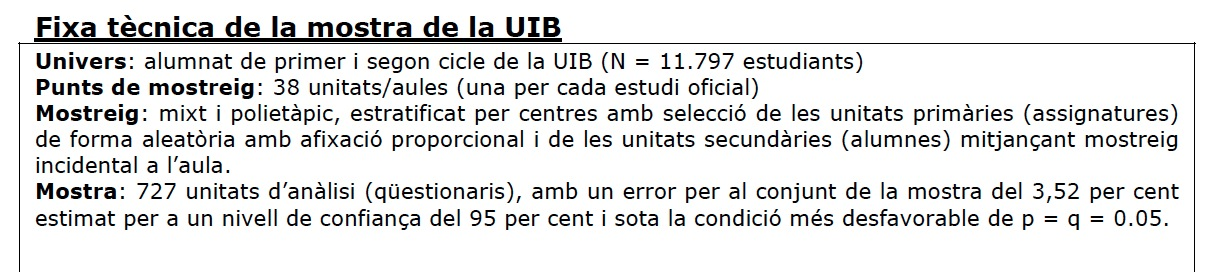
\includegraphics[width=1.1\linewidth]{plagiUIB2.jpg}
\end{center}


\end{frame}

\begin{frame}
\frametitle{``Poblaciones finitas''}

En este caso sí se da el efecto de \emph{población finita} cuando $N$ es relativamente pequeño
\medskip

Así que en esta situación, en las fórmulas que hemos propuesto para los intervalos de confianza  I.C. para $\mu$ o $p$ hay que multiplicar el error estándar o el error muestral por el factor corrector de población finita
$$
\sqrt{\frac{N-n}{N-1}}
$$

\end{frame}

\begin{frame}
\frametitle{``Poblaciones finitas''}

Consideremos  la situación siguiente  :
\begin{itemize}
\item  $X$ una población de  tamaño  $N$ que sigue una distribución con media   poblacional $\mu$ desconocida

\item $X_1,\ldots,X_n$ una m.a.\ sin reposición de $X$, con media   $\overline{X}$

\item  $n$ es grande 
\end{itemize}

\begin{block}{``Teorema''}
En estas  condiciones, se recomienda utilizar el intervalo de confianza de $(1-\alpha)\cdot 100\%$  para $\mu$ de una población normal con $\sigma$ conocida
$\mu$
$$
\left]\overline{X}-z_{1-\frac{\alpha}{2}}\frac{\sigma}{\sqrt{n}}\sqrt{\frac{N-n}{N-1}},\
    \overline{X}+z_{1-\frac{\alpha}{2}}\frac{\sigma}{\sqrt{n}}\sqrt{\frac{N-n}{N-1}}\right[
$$
\end{block}



\end{frame}




\begin{frame}
\frametitle{``Poblaciones finitas''}
\vspace*{-2ex}

Consideremos  la situación siguiente  :
\begin{itemize}
\item  $X$ una población de  tamaño  $N$ que sigue una distribución Bernoulli con $p$ desconocida

\item $X_1,\ldots,X_n$ una m.a.\ sin reposición de $X$, con $n$ muy grande  y con frecuencia relativa de éxitos $\widehat{p}_{X}$ lejos de los  extremos
\end{itemize}
\medskip

\begin{block}{``Teorema''}
En estas  condiciones, es recomienda tomar como  intervalo  de confianza  del $(1-\alpha)\cdot 100\%$ el parámetro $p$
$$
\begin{array}{l}
\displaystyle \left]\widehat{p}_{X}-z_{1-\frac{\alpha}{2}}\sqrt{\frac{\widehat{p}_{X}
(1-\widehat{p}_{X})}{n}}\sqrt{\frac{N-n}{N-1}}\right.,\\[1ex]
\hspace*{3cm}\displaystyle
\left.\widehat{p}_{X}+z_{1-\frac{\alpha}{2}}\sqrt{\frac{\widehat{p}_{X}
(1-\widehat{p}_{X})}{n}}\sqrt{\frac{N-n}{N-1}}\right[
\end{array}$$
\end{block}
\end{frame}


\begin{frame}
\frametitle{``Poblaciones finitas''}

\begin{block}{``Teorema''}
En las condiciones anteriores, para obtener un intervalo de confianza  del $(1-\alpha)\cdot 100\%$ para $p$ en el peor de los casos necesitaremos tomar una muestra de tamaño 
$$
n=\left\lceil\frac{Nz_{1-\frac{\alpha}{2}}^2}{A^2(N-1)+z_{1-\frac{\alpha}{2}}^2}\right\rceil
$$
\end{block}
\end{frame}

\begin{frame}
\frametitle{Ejemplo}
\vspace*{-5ex}

\begin{center}
\hspace*{-0.5cm}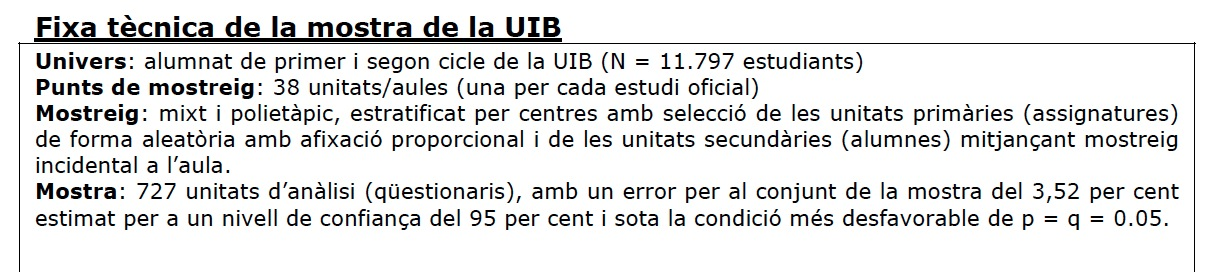
\includegraphics[width=1.1\linewidth]{plagiUIB2.jpg}
\end{center}

\blue{De la población total de estudiantes de grado de la UIB ¿cuántos hemos de escoger de manera aleatoria  y sin  reposición para estimar la proporción de los que han cometido plagio, con un error del 3.52\% y un nivel de confianza  del 95\%?}
%\pause

$$
n=\left\lceil\frac{11797\cdot 1.96^2}{0.0704^2\cdot 11796+1.96^2}\right\rceil=\lceil 727.3854\rceil=728
$$
\end{frame}

\end{document}

